\section{Fuzzy Clustering}

\begin{frame}
\frametitle{Fuzzy Clustering}

\pause

Dado $X = (x_1, x_2,..., x_k)$, con $k$ puntos de datos y $c$ clusters. \\

\pause
Definimos la función de pertenencia como:

\begin{equation}
    \begin{aligned}
        \mu_{ij} = \mu_i(x_j) \in [0, 1] \ \ \forall i = 1,...,c \land \forall j = 1,...,k
    \end{aligned}
\end{equation} 

\pause

De forma tal que:
%
\begin{equation}
    \begin{aligned}
        \sum_{i=1}^{c} \mu_i(x_j) = 1 \ \ \forall j = 1,...,k
    \end{aligned}
\end{equation} 

\note{
Es un método de clustering en el cual cada punto de los datos puede \textbf{pertenecer a más de un cluster}, mediante la asignación de valores de pertenencia a cada punto de nuestros datos por cada cluster que estemos buscando. Así, puntos cerca del borde de un cluster obtienen un bajo valor de pertenencia.
}

\end{frame}

\begin{frame}
\frametitle{Fuzzy Clustering}

Luego, definimos el conjunto de particiones difusas de la siguiente manera:

\begin{equation}
    \begin{aligned}
        M_{fc} = \{U \in \Re^{cxk} | U = [u_{ij}];u_{ij} \in [0, 1] \forall i, j; \sum_{i=1}^{c} u_{ij} = 1  \forall j; \sum_{j=1}^{k} u_{ij} > 0  \forall i \}
    \end{aligned}
\end{equation}

\pause

Función de error mínimo cuadrático:

\begin{equation}
    \begin{aligned}
        J_m(U, v) = \sum_{j=1}^{k} \sum_{i=1}^{c} (u_{ij})^m d_{ij}^2
    \end{aligned}
\end{equation} 

\begin{itemize}
    \item $d_{ij}$: Distancia Euclidiana entre el elemento $x_j$ y el centro del cluster $i$
    \item $U \in M_{fc}$: Contiene todos los pesos $u_{ij}$ asociados a las distancias cuadradas
    \item $v$: El vector centro de cada cluster
    \item $m$: Valor de fuzzines
\end{itemize}

\note{
%- Partición difusa: La caracterización de la participación de cada muestra en todos los clusters a partir de un valor de pertenecía que va de $[0, 1]$. Estas particiones difusas se representan con una matriz, asociando cada fila a uno de los $c$ clusters y cada columna a uno de los elementos de $X$, de forma tal que el valor en la fila $i$ y la columna $j$ indique la pertenencia del elemento $j$ al cluster $i$ \\
- Que representa una particion difusa (sus elementos)
\pause

- Podemos \textbf{traducir el problema} de FCM a buscar una particion difusa (es decir, una matriz perteneciente al conjunto descrito arriba) \textbf{"optima"}
}
\end{frame}


\begin{frame}
\frametitle{Fuzzy Clustering}

Algoritmo:

\begin{enumerate}
  \item <1-> Fijar $c$, $k$ y $m$. Elegir una matriz inicial $U^{(0)}\in M_{fc}$
  \item <2-> Calcular los centros de los clusters como $v_{i}={\frac {\sum \limits _{j=1}^{k}(u_{ij})^{m}x_{j}}{\sum \limits _{j=1}^{k}(u_{ij})^{m}}};1\leq i\leq c$
  \item <3-> Actualizar la matriz de partición difusa $U = [uij]$ con $u_{ij}=(\sum \limits _{n=1}^{c}({\frac {d_{ij}}{d_{nj}}})^{\frac {2}{m-1}})^{-1};1\leq j\leq k;1\leq i\leq c$
  \item <4-> Si se alcanzo la máxima cantidad de iteraciones, o la diferencia de la matriz U con respecto a la iteración anterior es menor al error mínimo dado, el algoritmo termina. Caso contrario, vuelve al paso 2.
\end{enumerate}

\note{
- $m \rightarrow 1 = kmeans$, $m \rightarrow \infty =$ el mismo valor de pertenencia para todos los clusters \\
- Una vez terminado de correr el algoritmo, \textbf{etiquetamos} cada dato de nuestro conjunto con el cluster cuyo valor en la \textbf{partición difusa sea mayor}. \\
}

\end{frame}



\begin{frame}
\frametitle{Librería utilizada}

\begin{center}
    
\includegraphics[width=7cm]{fuzzy clustering/figures/scikit-fuzzy.png}
    \href{https://pythonhosted.org/scikit-fuzzy/}{https://pythonhosted.org/scikit-fuzzy/}
\end{center}

\end{frame}


\begin{frame}
\frametitle{Abadi: Búsqueda de $m$}


\begin{columns}
\column{0.4\textwidth}

\begin{center}
    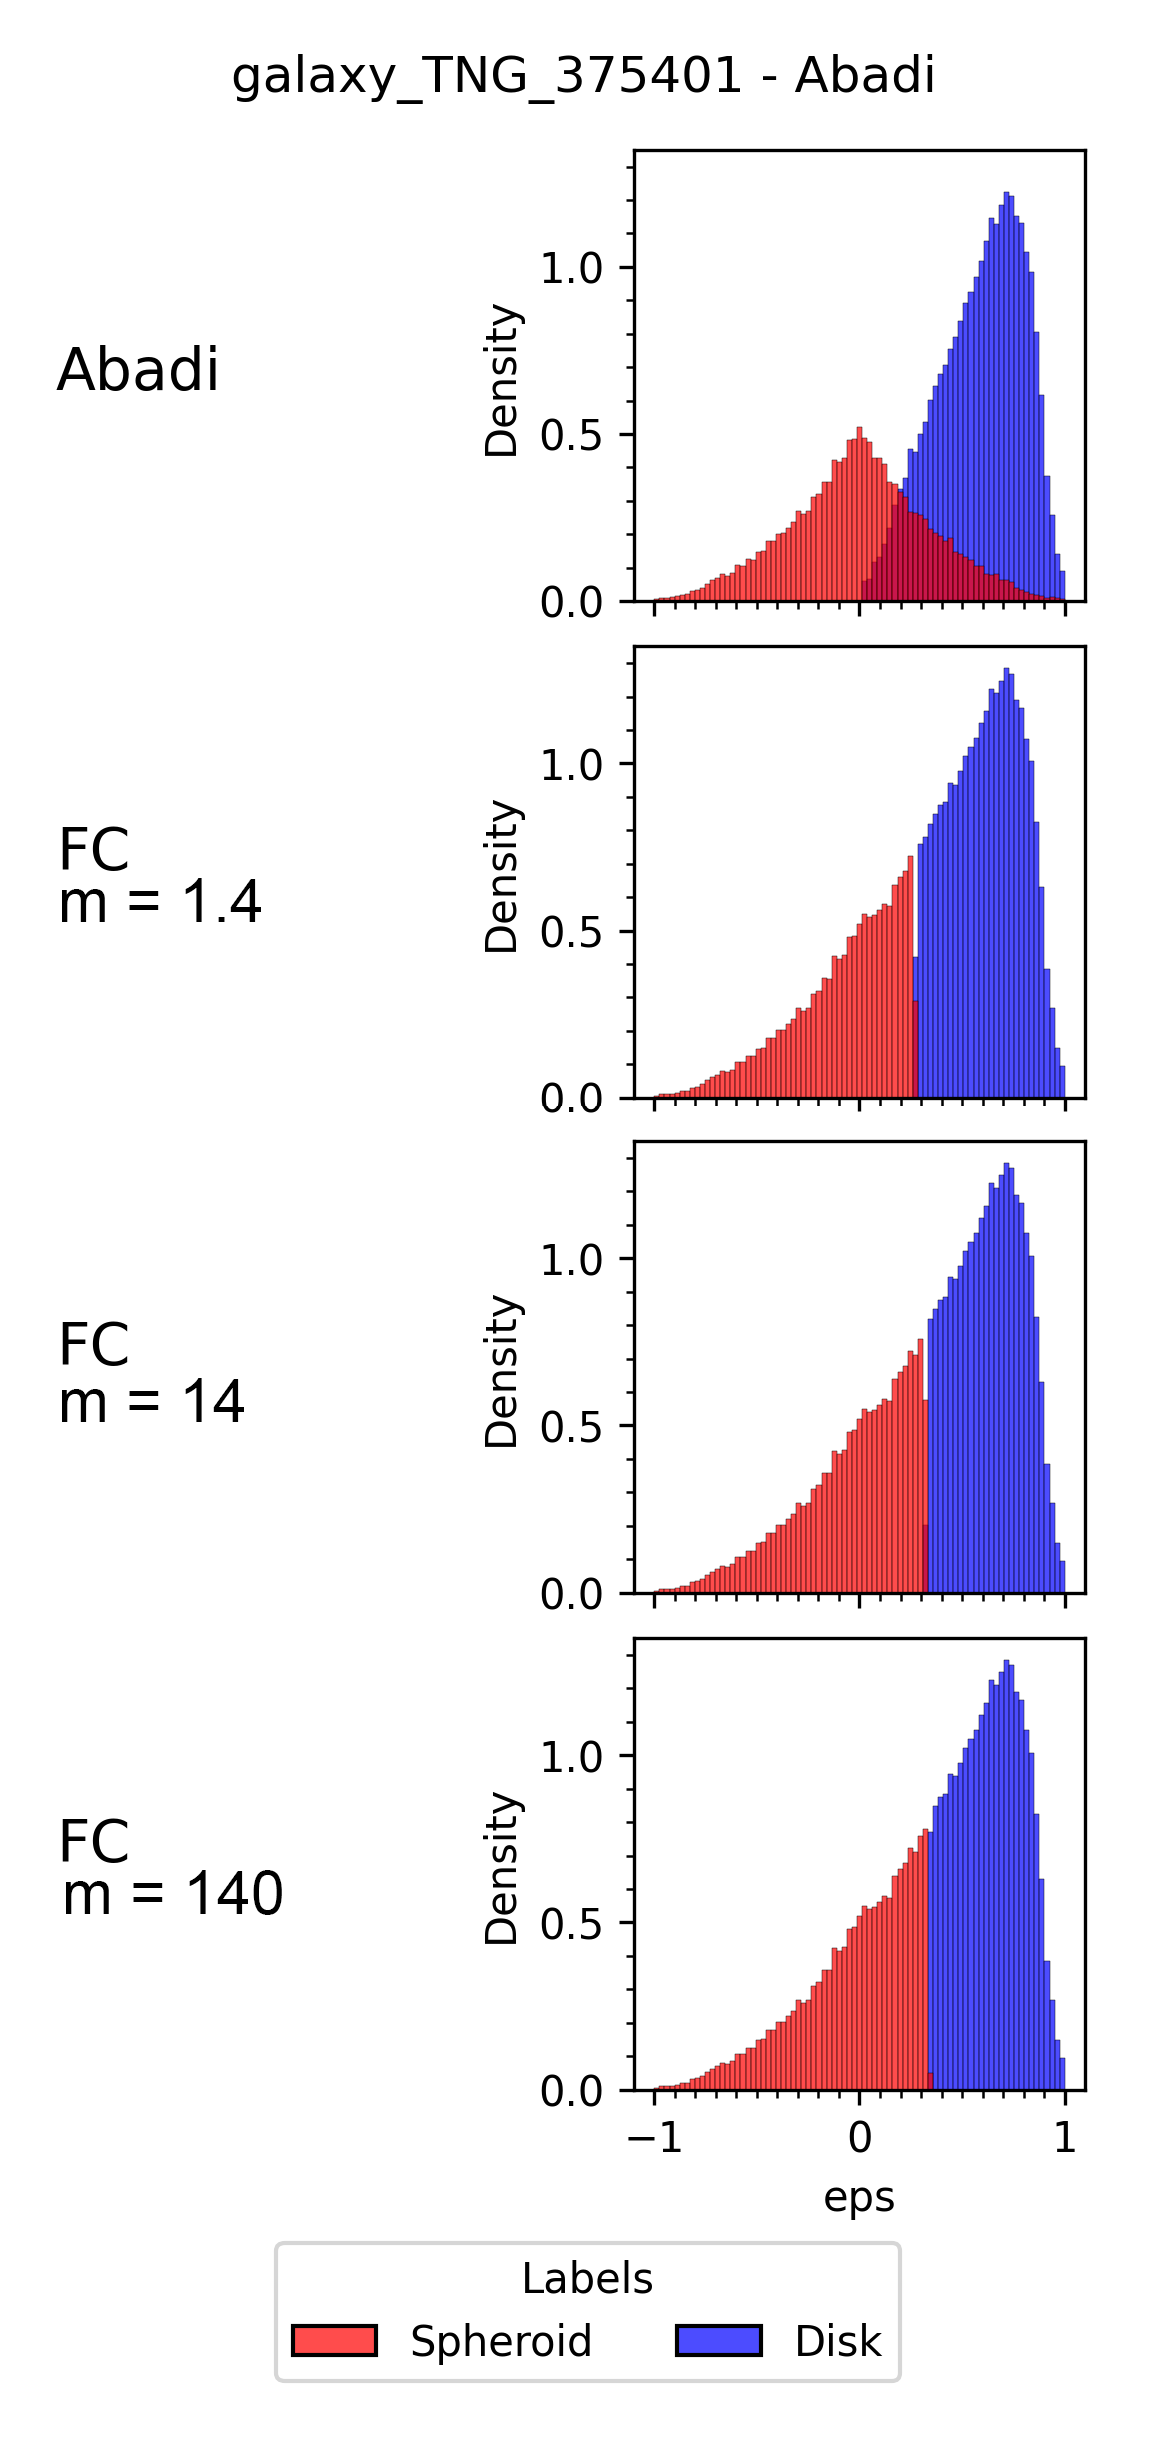
\includegraphics[width=3.8cm]{fuzzy clustering/figures/galaxy_TNG_375401 - Abadi - circ histogram fuzzines comparison.png}
\end{center}

\column{0.6\textwidth}

\begin{table}
\centering
\begin{tabular}{|c|c|}
\hline
Fuzziness&Centro de Esferoide\\
\hline
$1.4$ & $-0.078$\\
\hline
$14$ & $0.008$\\
\hline
$140$ & $0.027$\\
\hline
\end{tabular}

\end{table}

%\pause

%MAX VALUE \texttt{float64} = $2.225 \times 10^{-308}$ \\
%Q1 $u_{ij}$ (con $i$ = Disk) = $7.56 \times 10^{-5}$ \\
%m = $75$

\end{columns}

\note{
%- recordamos que como usamos una sola feature no vamos a tener mas informacion para mezclar los resultados con fuzzines\\
%- porque se \textbf{mueve la recta hacia la derecha} al aumentar m? Mirar la segunda ecuacion, aumentar m decrementa el peso que tiene xj para calcular el centro del cluster. \\
%- En la libreria los valores de pertenencia estan guardados en float64. Si separamos en quartiles ordenando por el valor de pertenencia de cada componente nos encontramos con que Q1 del disco tiene ese valor, que no es lo suficientemente chico, pero un m de 75 basta con hacer que sea menor al valor de arriba. \\
%- Aporte los \textbf{puntos más alejados de cada cluster} será nulos para el \textbf{segundo paso del algoritmo}, entonces las partículas que se encuentran más cercanas al extremo izquierdo de la recta no afectarán al cálculo del centro del cluster del Esferoide. Mayoria de estas particulas en el extremo izquierdo. Algo similar sucede con el Disco. \\
%- Partículas que se encuentren entre el centro del Esferoide y el Disco en la recta y las cuales antes tenían un valor de pertenencia al Disco mayor que el valor de pertenencia al Esferoide, pasen a formar parte del Esferoide, moviendo la línea de corte hacia la derecha en el proceso. \\
%- Entre más grande es el valor de fuzziness, la diferencia entre los puntos que pasaran a no formar parte del cálculo de centros de clusters entre el Esferoide y el Disco se incrementará aún más, moviendo el corte hacia la derecha en la misma medida \\
Aumentar m movia la \textbf{linea de corte} hacia la \textbf{derecha}.
}



\end{frame}





\begin{frame}
\frametitle{Abadi: Detección de 2 componentes}

Concluimos en usar:
\begin{enumerate}
    \item $m$ = 1.4
    \item Error mínimo = $0.00005$
    \item Iteraciones máximas =  $1000$
\end{enumerate}

\begin{center}
    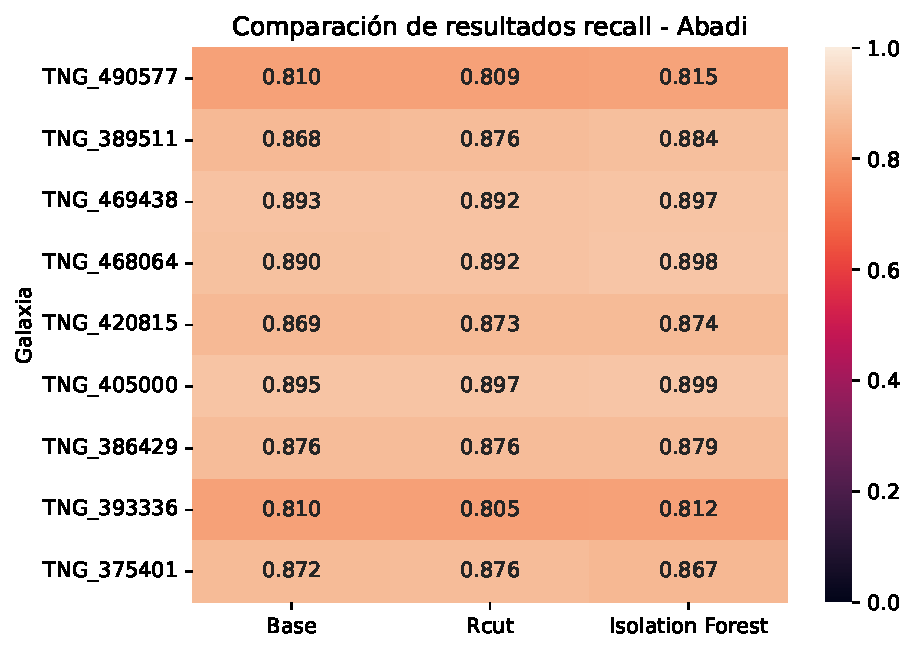
\includegraphics[width=8cm]{fuzzy clustering/figures/abadi - recall.pdf}
\end{center}

%ver mejor?
\note{
- Dado el dominio de resultados posibles, pasamos a elegir un \textbf{valor de fuzziness que acerque la linea de corte} al punto promedio en donde la densidad del Disco supera a la del Esferoide en todas las galaxias de nuestro dataset \\
- \textbf{Similar con CJ}, fuzzy es bueno al buscar 2 clusters entendiendo sus limitaciones?
}

\end{frame}




\begin{frame}
\frametitle{Abadi: Eliminación de outliers}

\begin{center}
    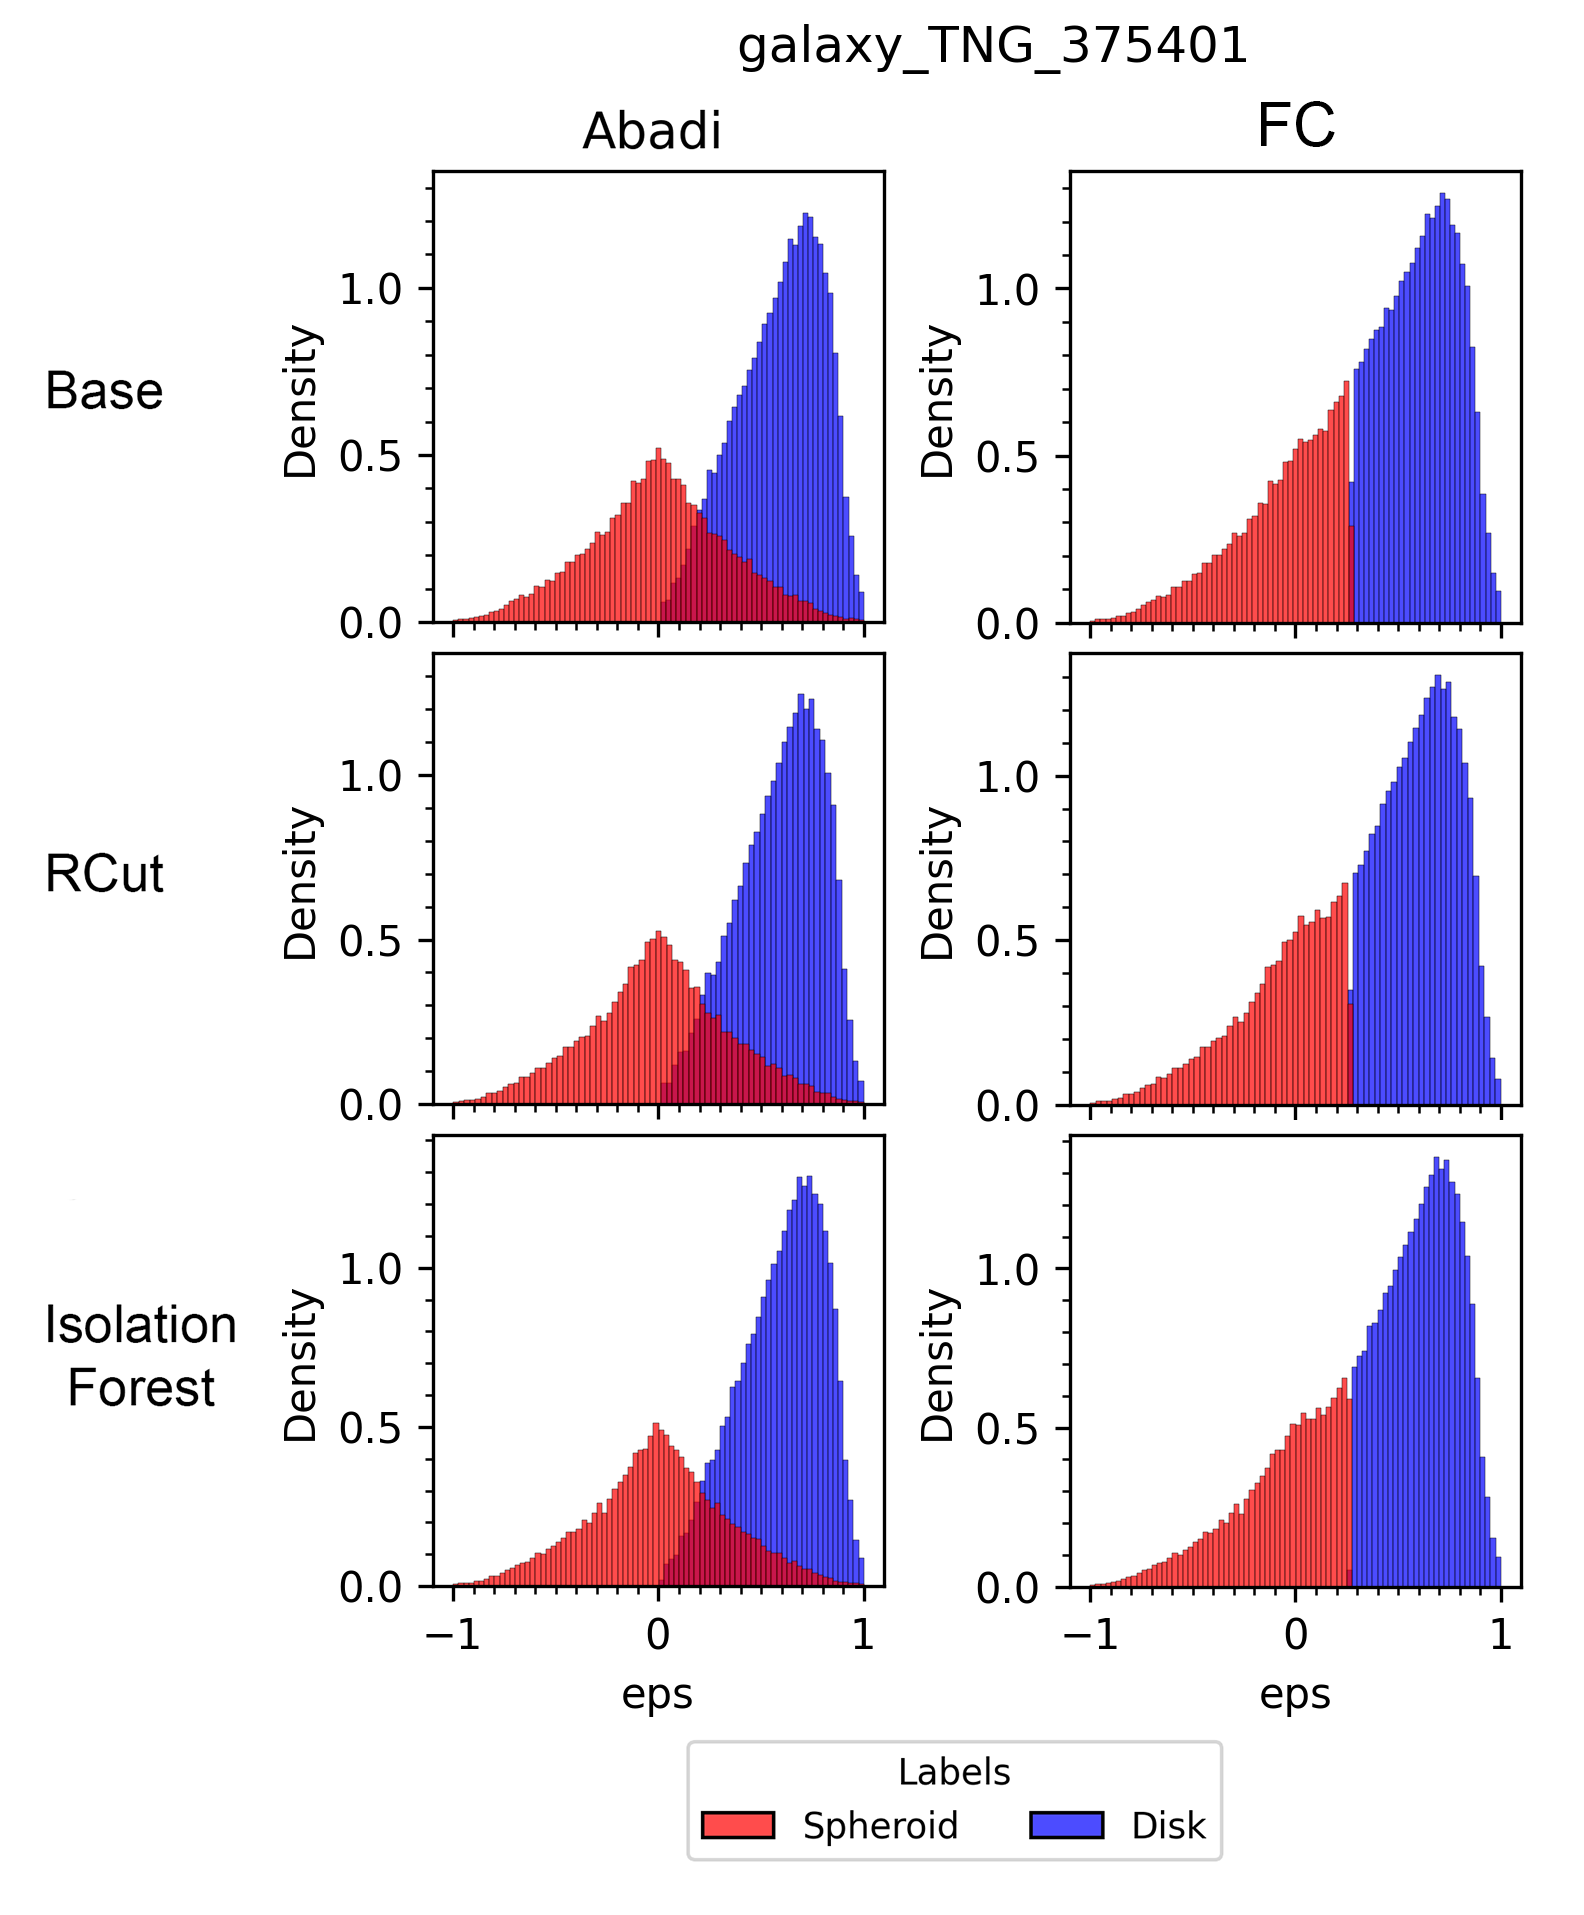
\includegraphics[width=6.5cm]{fuzzy clustering/figures/galaxy_TNG_375401 - Abadi - outlier removal comparison.png}
\end{center}

\note{
- Aplicar \gls{IF} y \gls{RCUT} \textbf{apenas si modifican} los conjuntos encontrados de forma perceptible \\
- Esto se debe a que Fuzzy clustering es un método robusto dado que \textbf{limita el impacto de los outliers} al calcular los centros de los clusters, por lo que sacarlos apenas tiene efecto
}

\end{frame}

\iflong
\begin{frame}
\frametitle{Abadi: Eliminación de outliers}

\begin{center}
    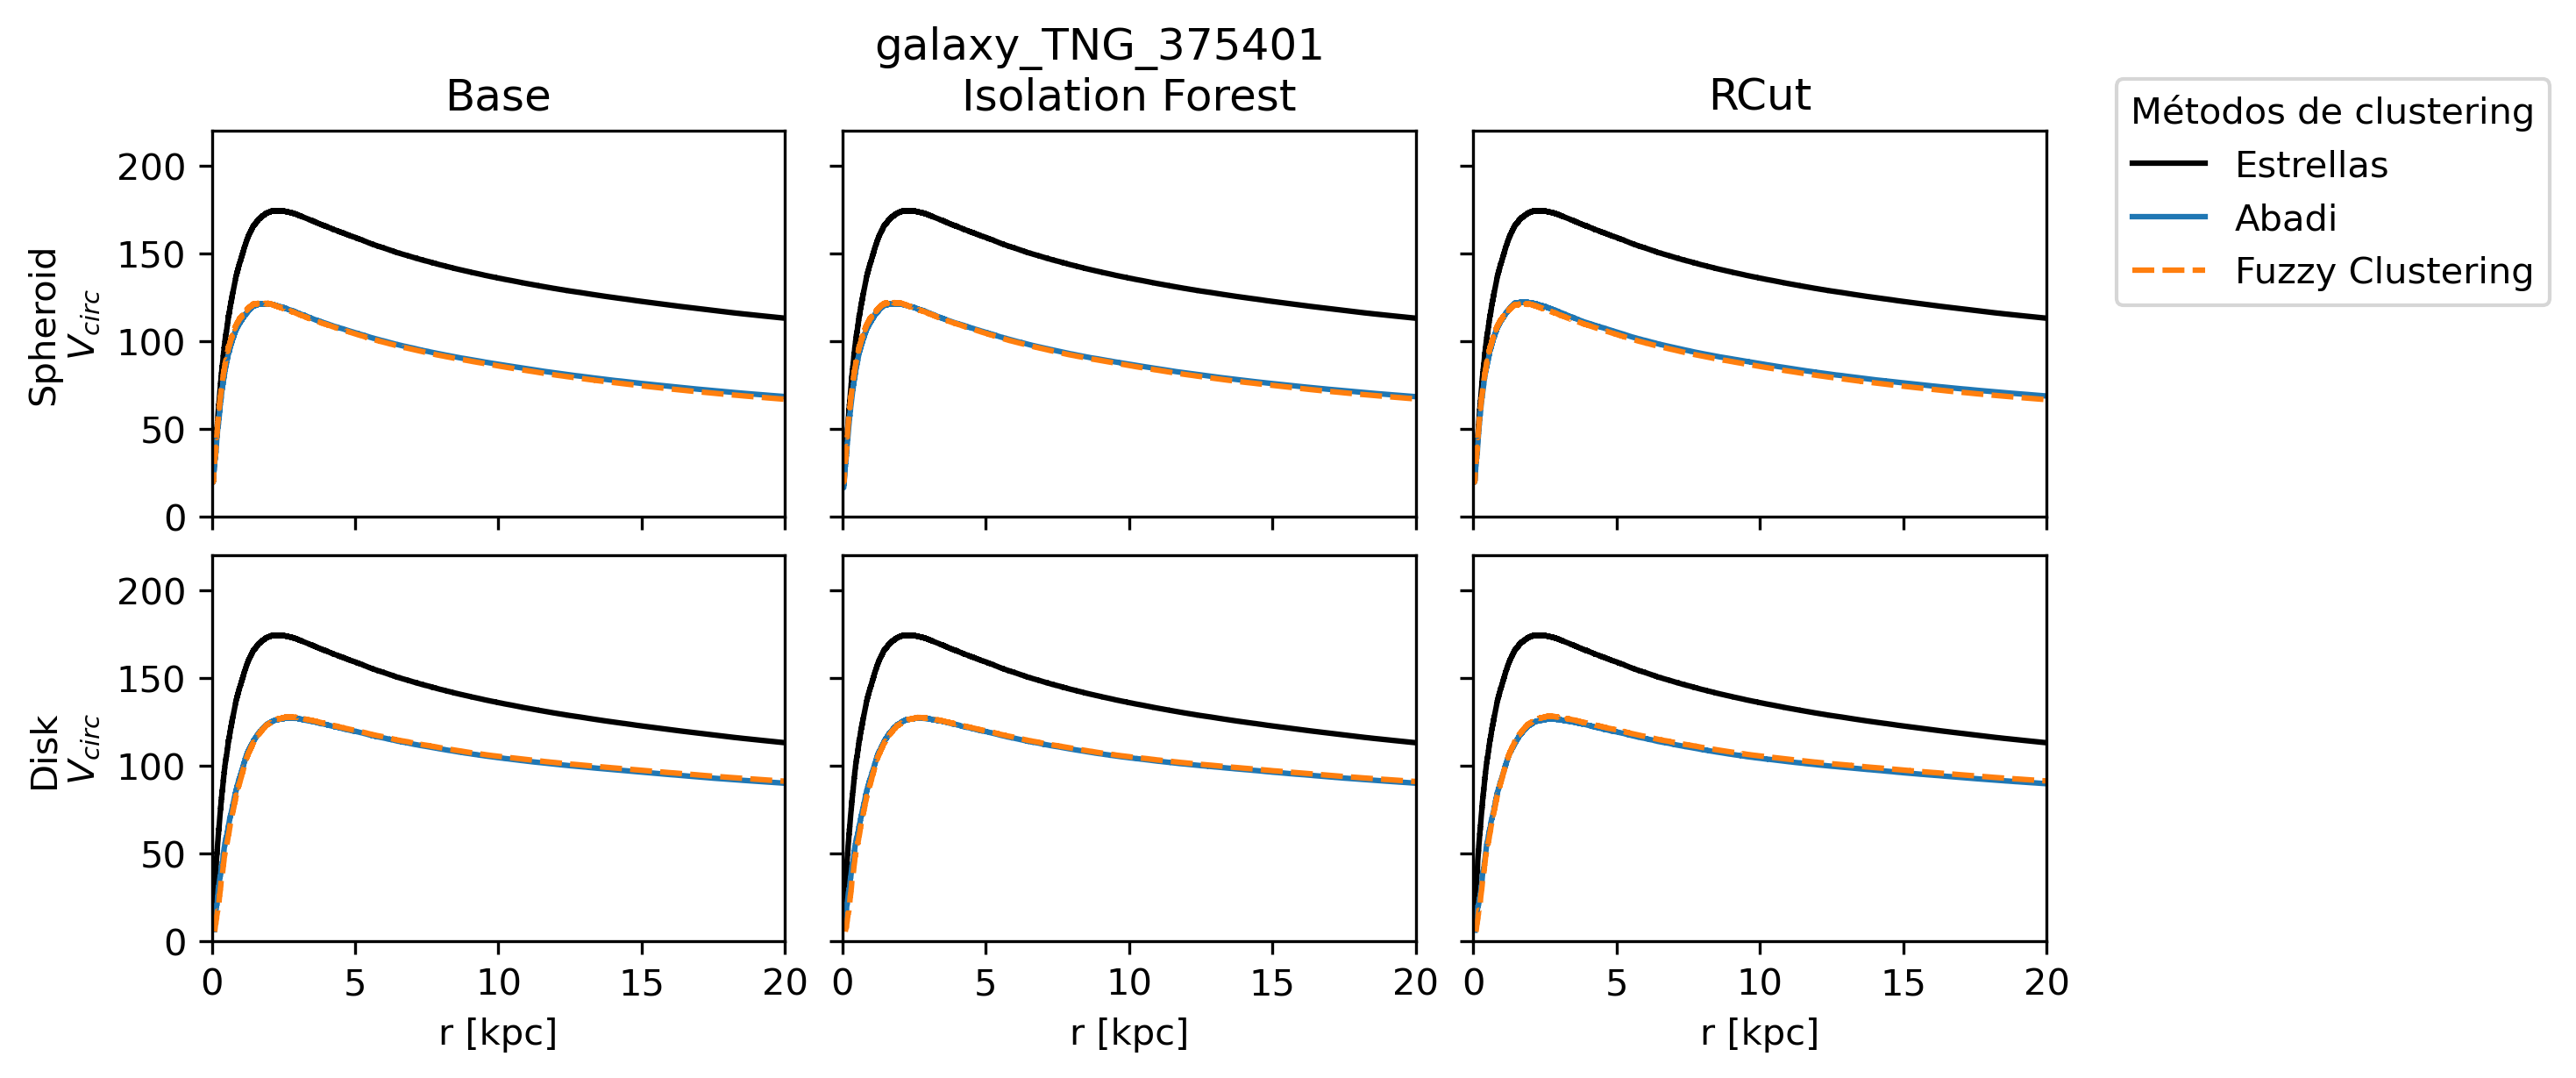
\includegraphics[width=12cm]{fuzzy clustering/figures/galaxy_TNG_375401 - Abadi - circ_velocity.png}
\end{center}

\end{frame}
\fi


\begin{frame}
\frametitle{AGMM: Detección de $>=$2 componentes}

\begin{enumerate}
    \item $m$ = 3
    \item Error mínimo = $0.00005$
    \item Iteraciones máximas =  $1000$
\end{enumerate}

\begin{center}
    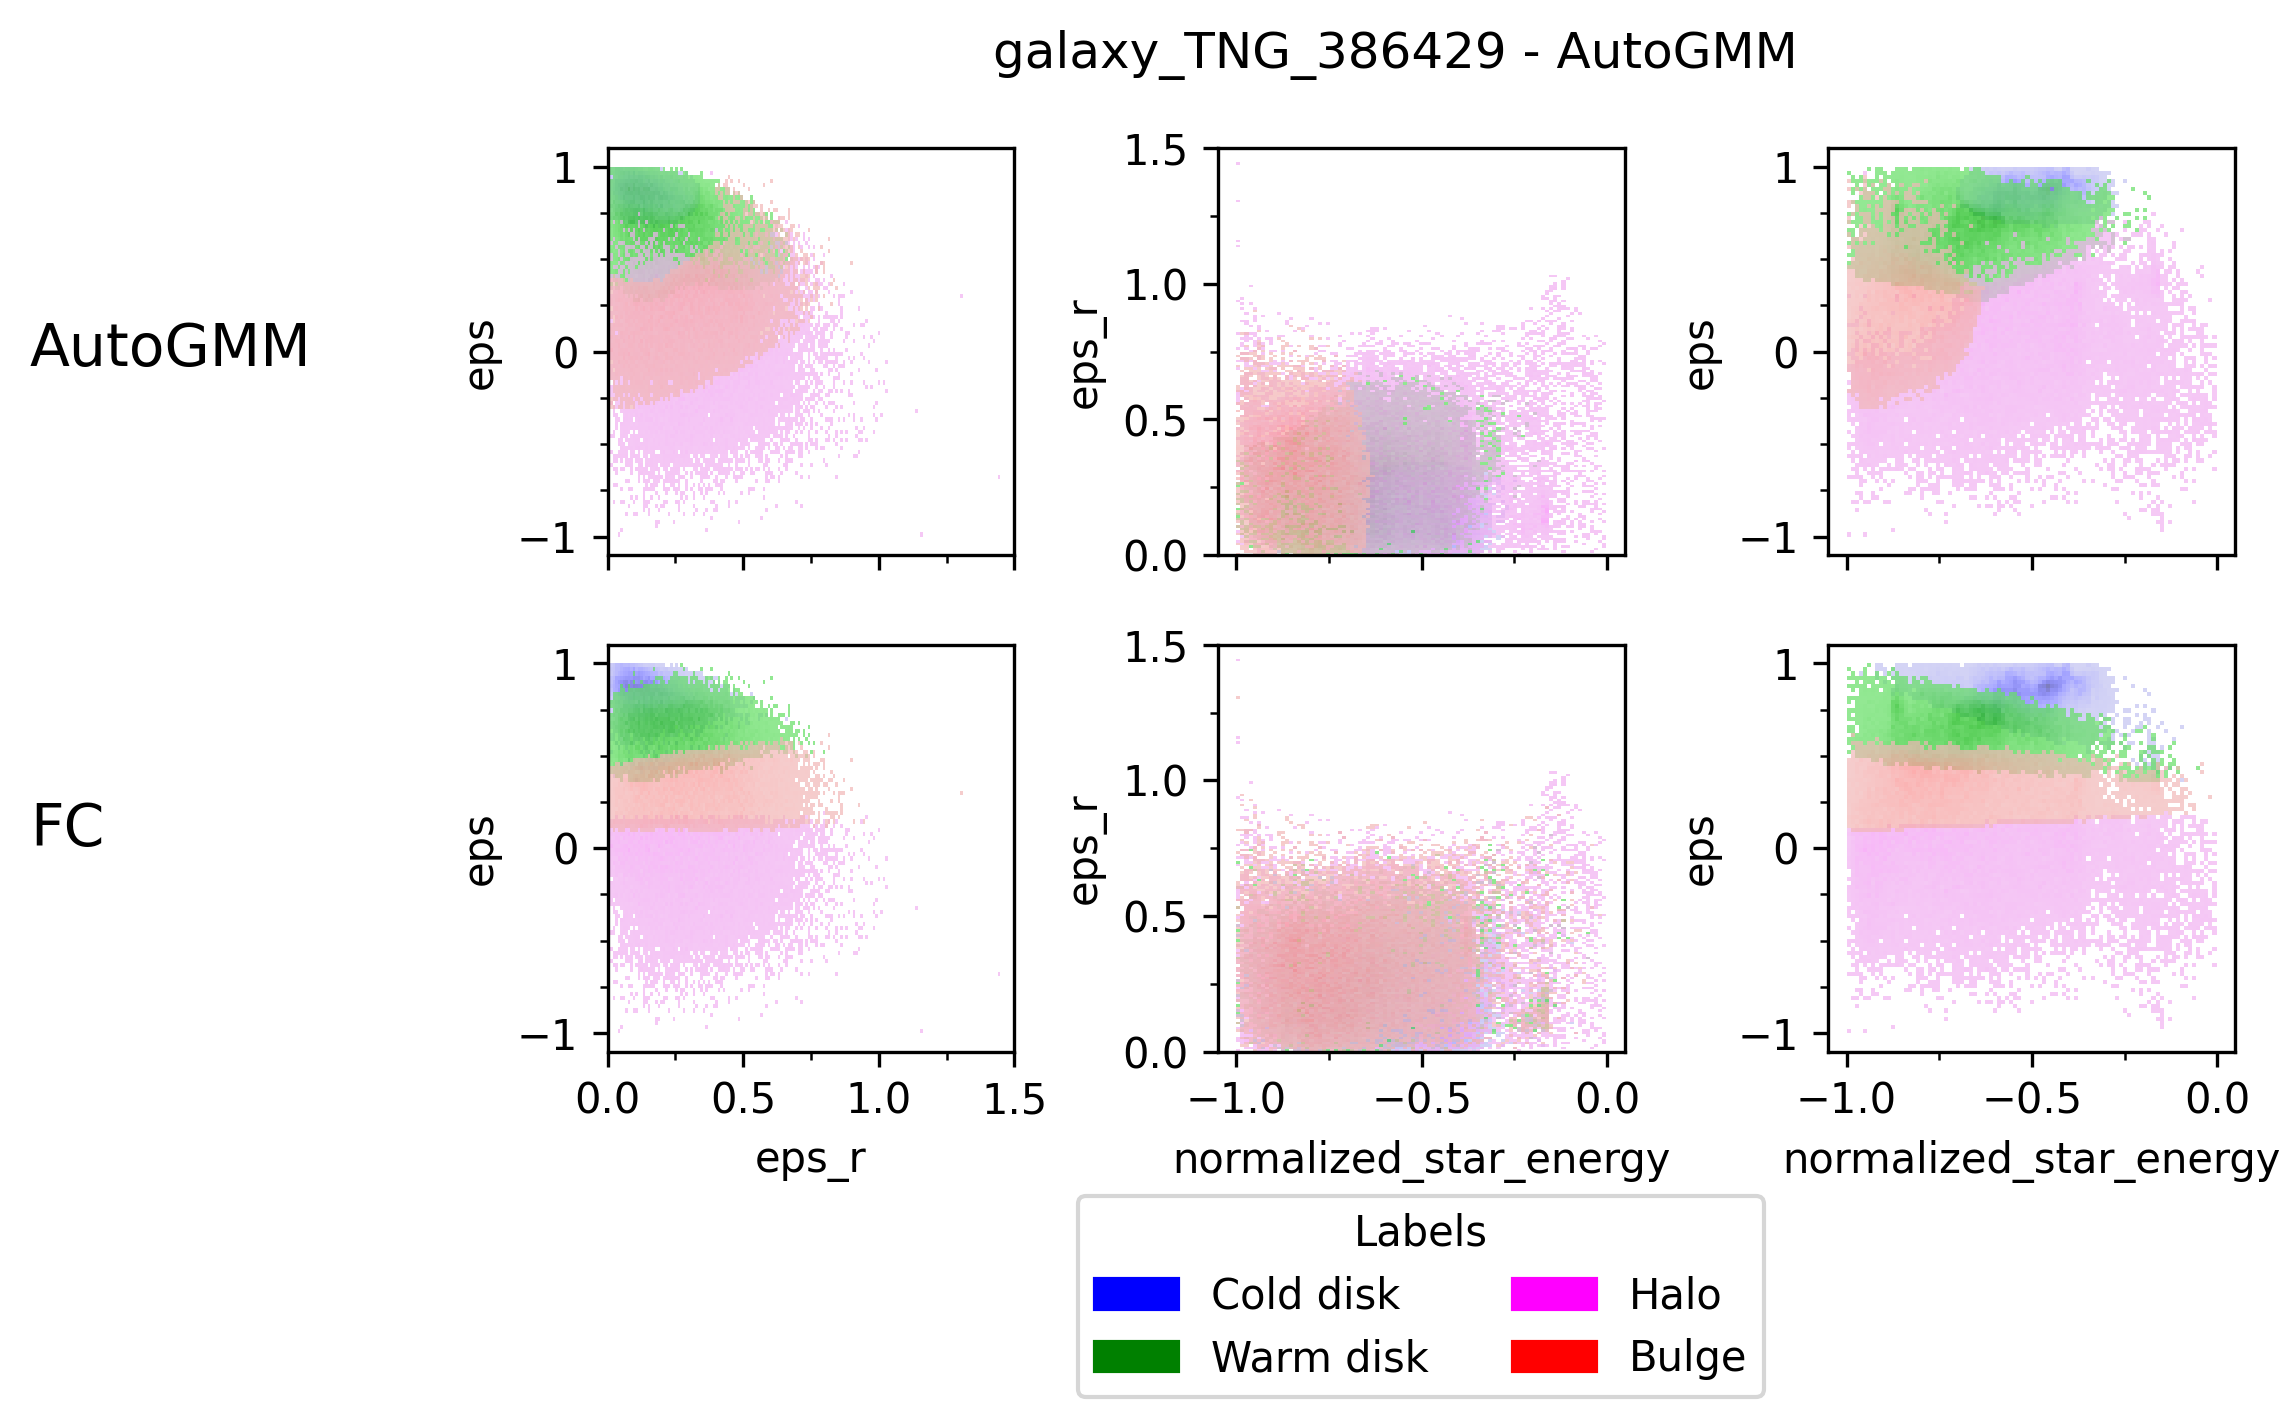
\includegraphics[width=10cm]{fuzzy clustering/figures/galaxy_TNG_386429 - circ scatterplot.png}
\end{center}
\note{
- \textbf{busqueda de m} ahora tiene el \textbf{efecto esperado} al usar mas features \\
%- lo que nos deja mas cercano a agmm, mantendremos el resto de los valores \\
- Similar a CJ, los resultados son bastante \textbf{unidimencionales} \\
- Creemos que fue por una \textbf{sobre reelevancia de features}. Aunque eps nos sirva para identificar ambos discos, necesitamos utilizar mejor \textbf{normalized\_star\_energy} para identificar el \textbf{bulge} y el \textbf{halo}, como se puede ver en el siguiente histograma (otra diapo) \\
}

\end{frame}


\begin{frame}
\frametitle{AGMM: Detección de $>=$2 componentes}

\begin{center}
    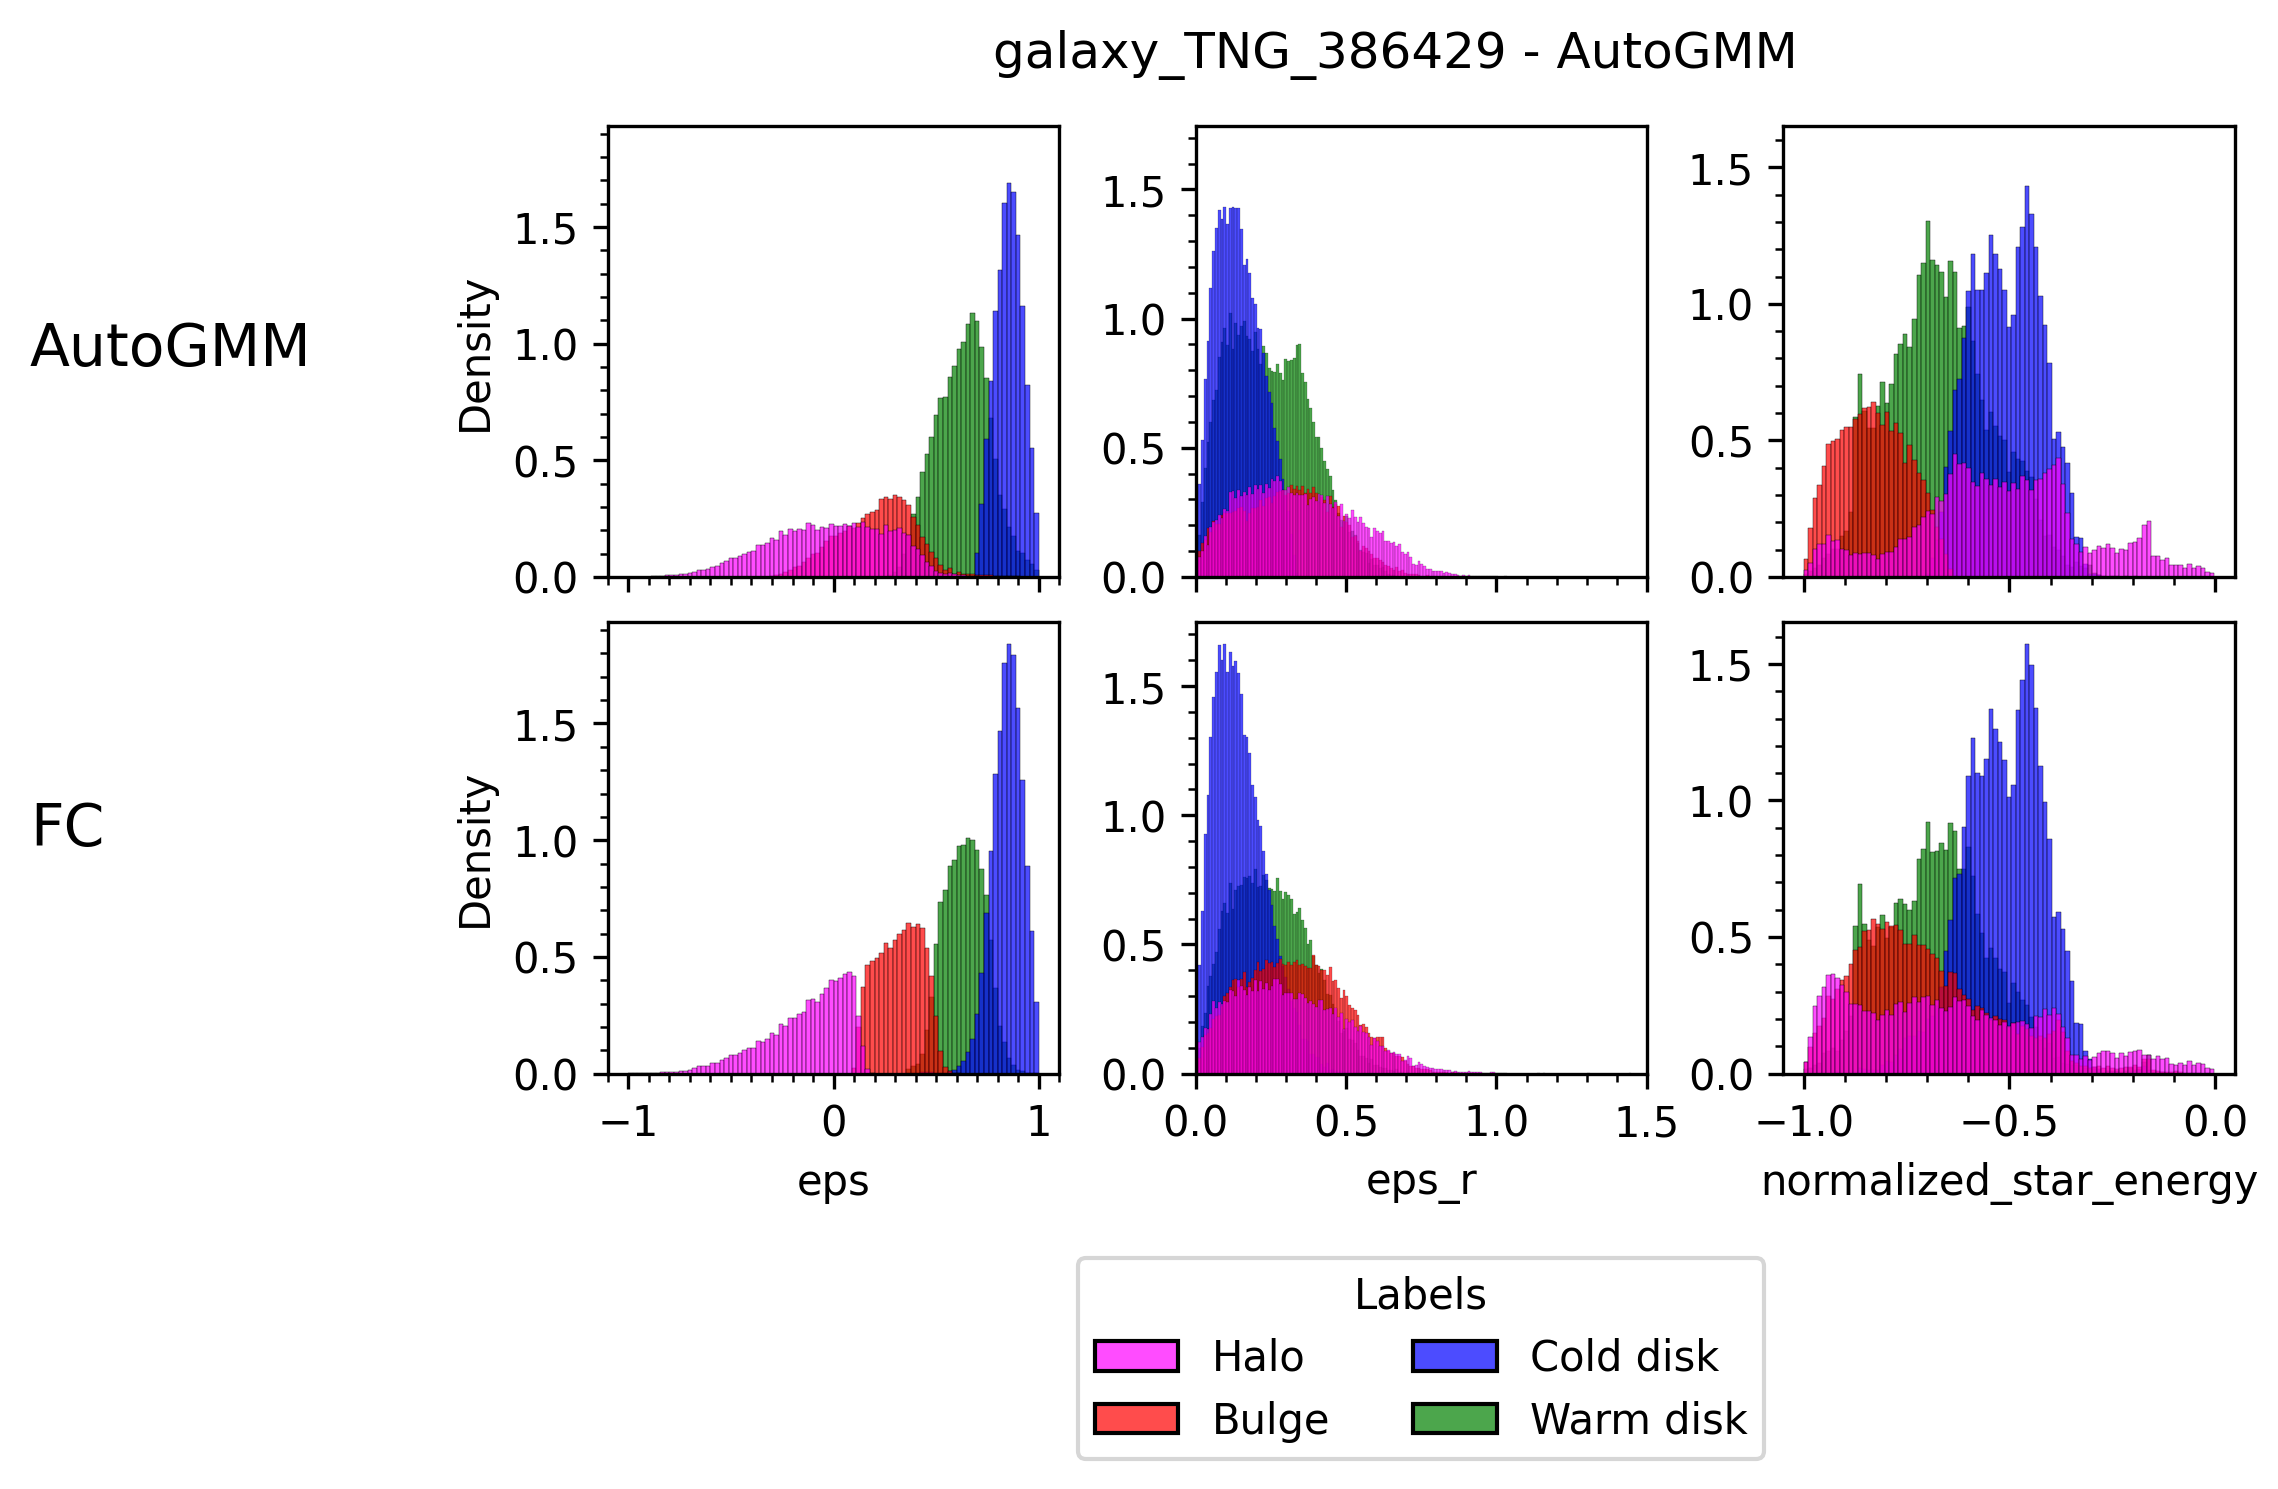
\includegraphics[width=12cm]{fuzzy clustering/figures/galaxy_TNG_386429 - circ histogram.png}
\end{center}

\note{
- Volvemos al \textbf{tercer paso del algo}, deriva el \textbf{valor de pertenencia} de cada partícula con cada cluster a partir de la \textbf{distancia} de ésta hacia el \textbf{centro de cada cluster}. \\
%- Sin embargo, observando las distribuciones de las partículas estelares podemos apreciar los \textbf{rangos de valores} que una partícula puede tener en \textbf{cada feature} (siguiente diapo)
%ponemos tabla?
%- Tabla: centro de los clusters encontrados por FCM estan mas o menos cerca de los encontrados por AGMM \\
}

\end{frame}




\begin{frame}
\frametitle{AGMM: Detección de $>=$2 componentes}
% explicar el tamaño cubierto por cada eje
\begin{center}
    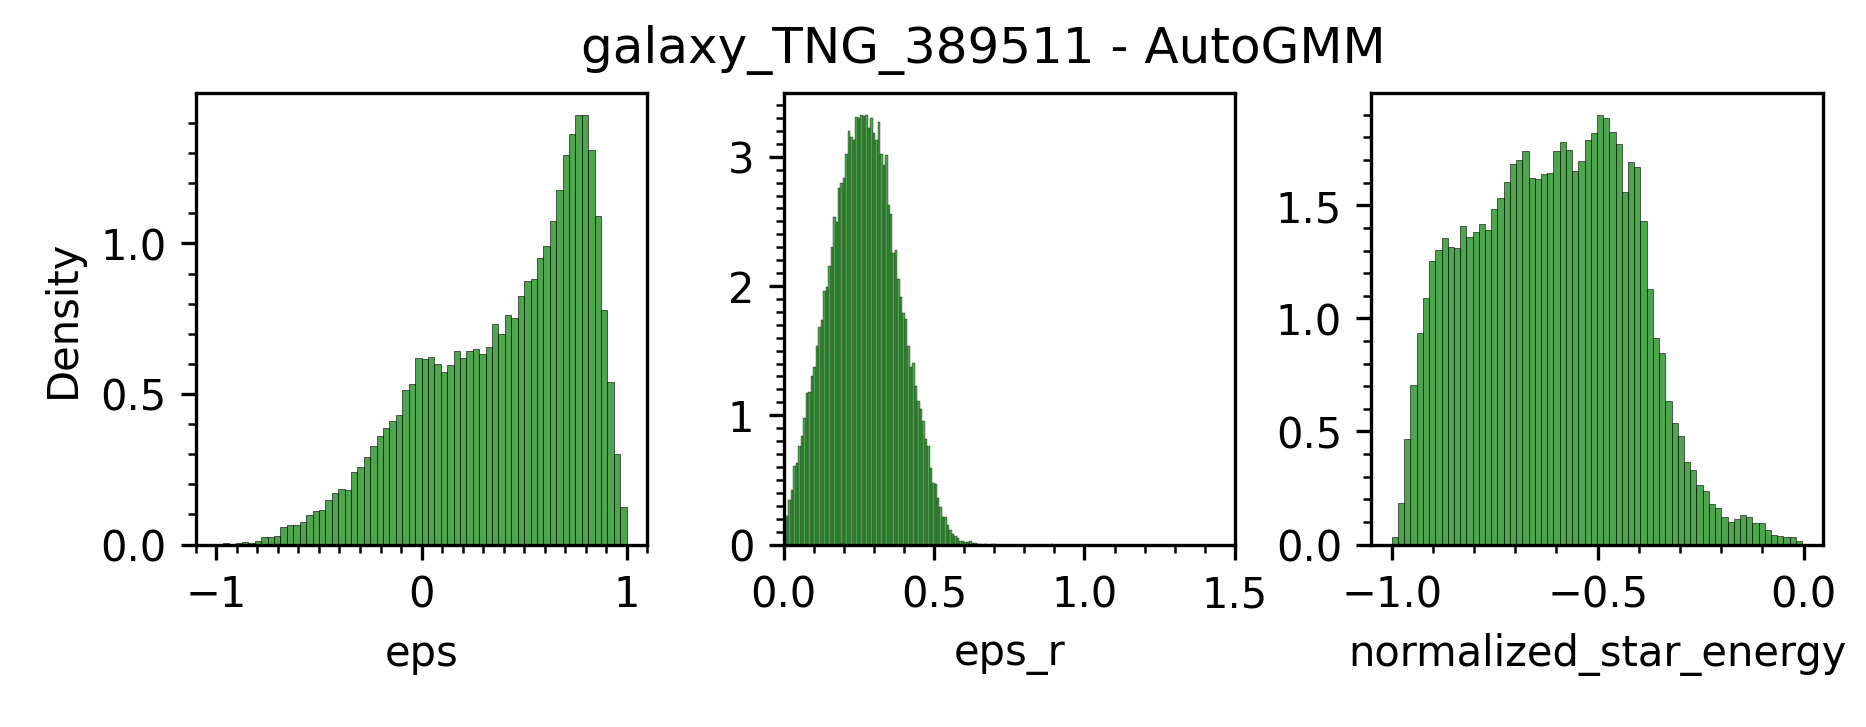
\includegraphics[width=12cm]{fuzzy clustering/figures/galaxy_TNG_389511 - circ histogram - features.png}
\end{center}

\note{
- Los valores de $eps$ tienen un rango $[-1, 1]$, mientras que el rango de los valores de $normalized\_star\_energy$ es $[-1, 0]$ y el de $eps\_r$ $[0, 1.5]$ (aunque a fines prácticos suele ser $[0, 1]$, incluso menor como se ve aca). \\
- Esto implica que haya \textbf{altas probabilidades} de que la \textbf{distancia} entre un punto a un cluster (y por consuecuente su \textbf{valor de pertenencia}) resulte fuertemente \textbf{dominado por eps}. \\
% Nuevamente, normalized star energy podria ayudar a diferenciar bulge y halo bastante \\
% eps_r no ayuda mucho \\
%- Curiosamente, podemos ver el efecto que tiene $normalized\_star\_energy$ sobre los valores de pertenencia, con las \textbf{lineas separatorias} en eps vs normalized star energy \textbf{un tanto inclinadas}. \\
%- Dicha inclinacion proviene del (leve) \textbf{aporte que hace la feature} de normalized star energy sobre el valor de pertenencia de las particulas. \\
}

\end{frame}


\iflong
\begin{frame}
\frametitle{AGMM: Detección de $>=$2 componentes}
\begin{center}
    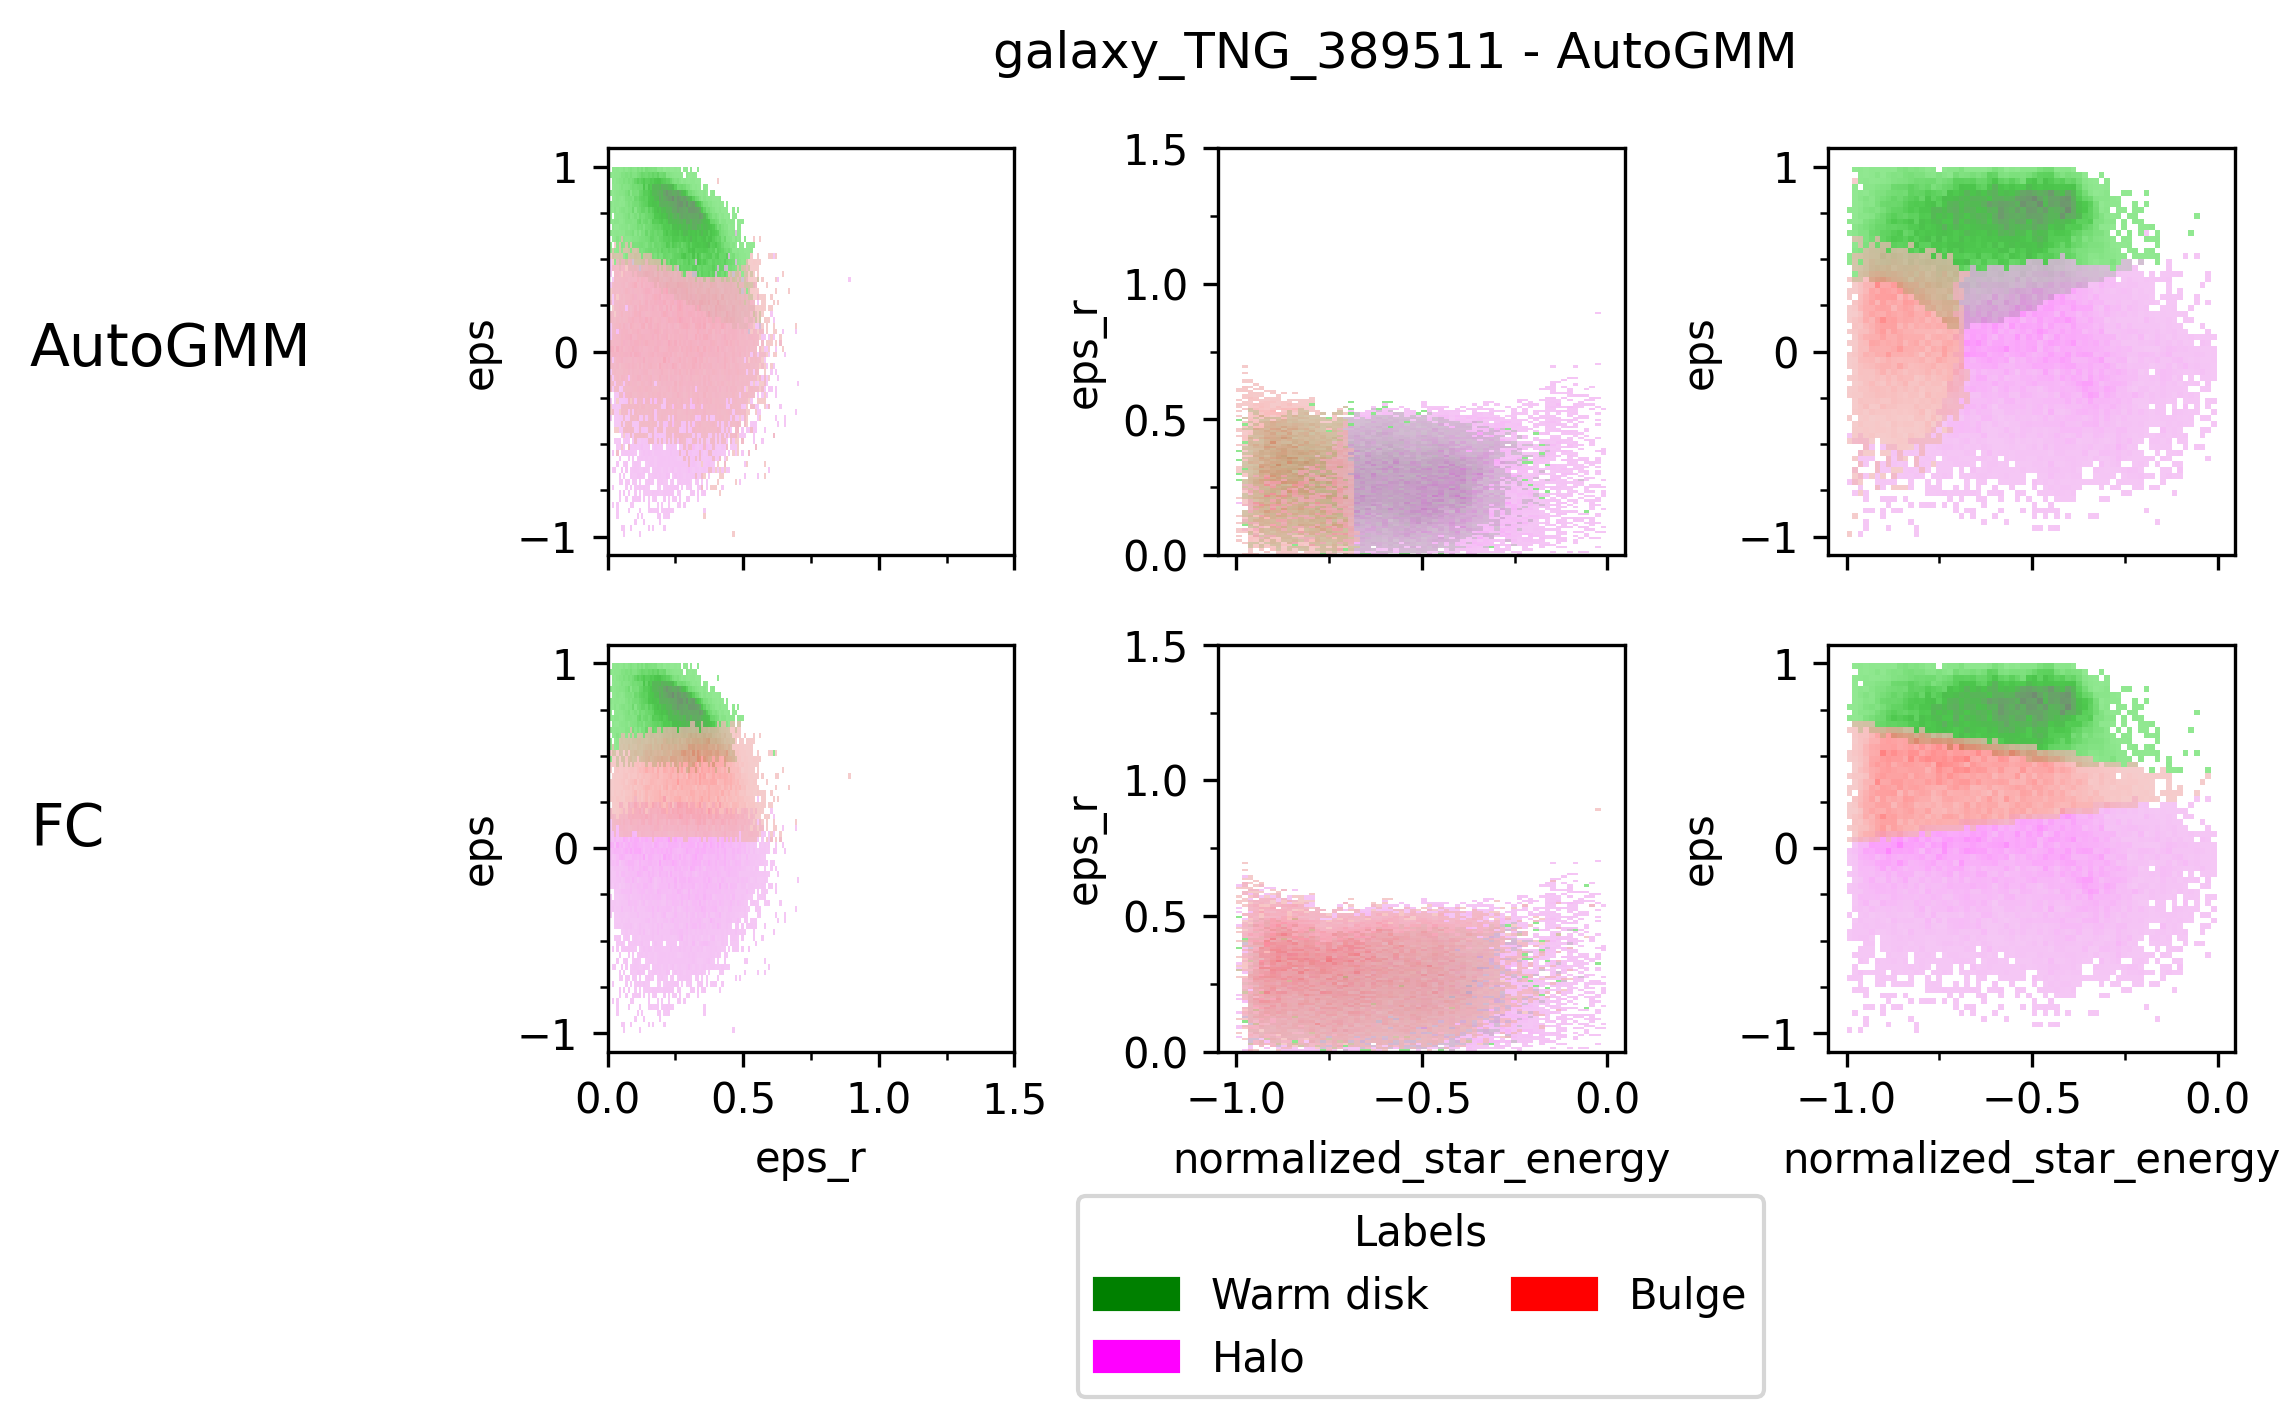
\includegraphics[width=12cm]{fuzzy clustering/figures/galaxy_TNG_389511 - circ scatterplot.png}
\end{center}

\note{
- Curiosamente, podemos ver el efecto que tiene $normalized\_star\_energy$ sobre los valores de pertenencia, con las lineas separatorias en eps vs normalized star energy un tanto inclinadas. \\
- Dicha inclinacion proviene del (leve) aporte que hace la feature de normalized star energy sobre el valor de pertenencia de las particulas. \\
- nulo aporte de eps_r en FCM, fijate lo recta que son las divisiones vs. eps \\
}

\end{frame}
\fi

\iflong
\begin{frame}
\frametitle{AGMM: Detección de $>=$2 componentes}


\begin{center}
    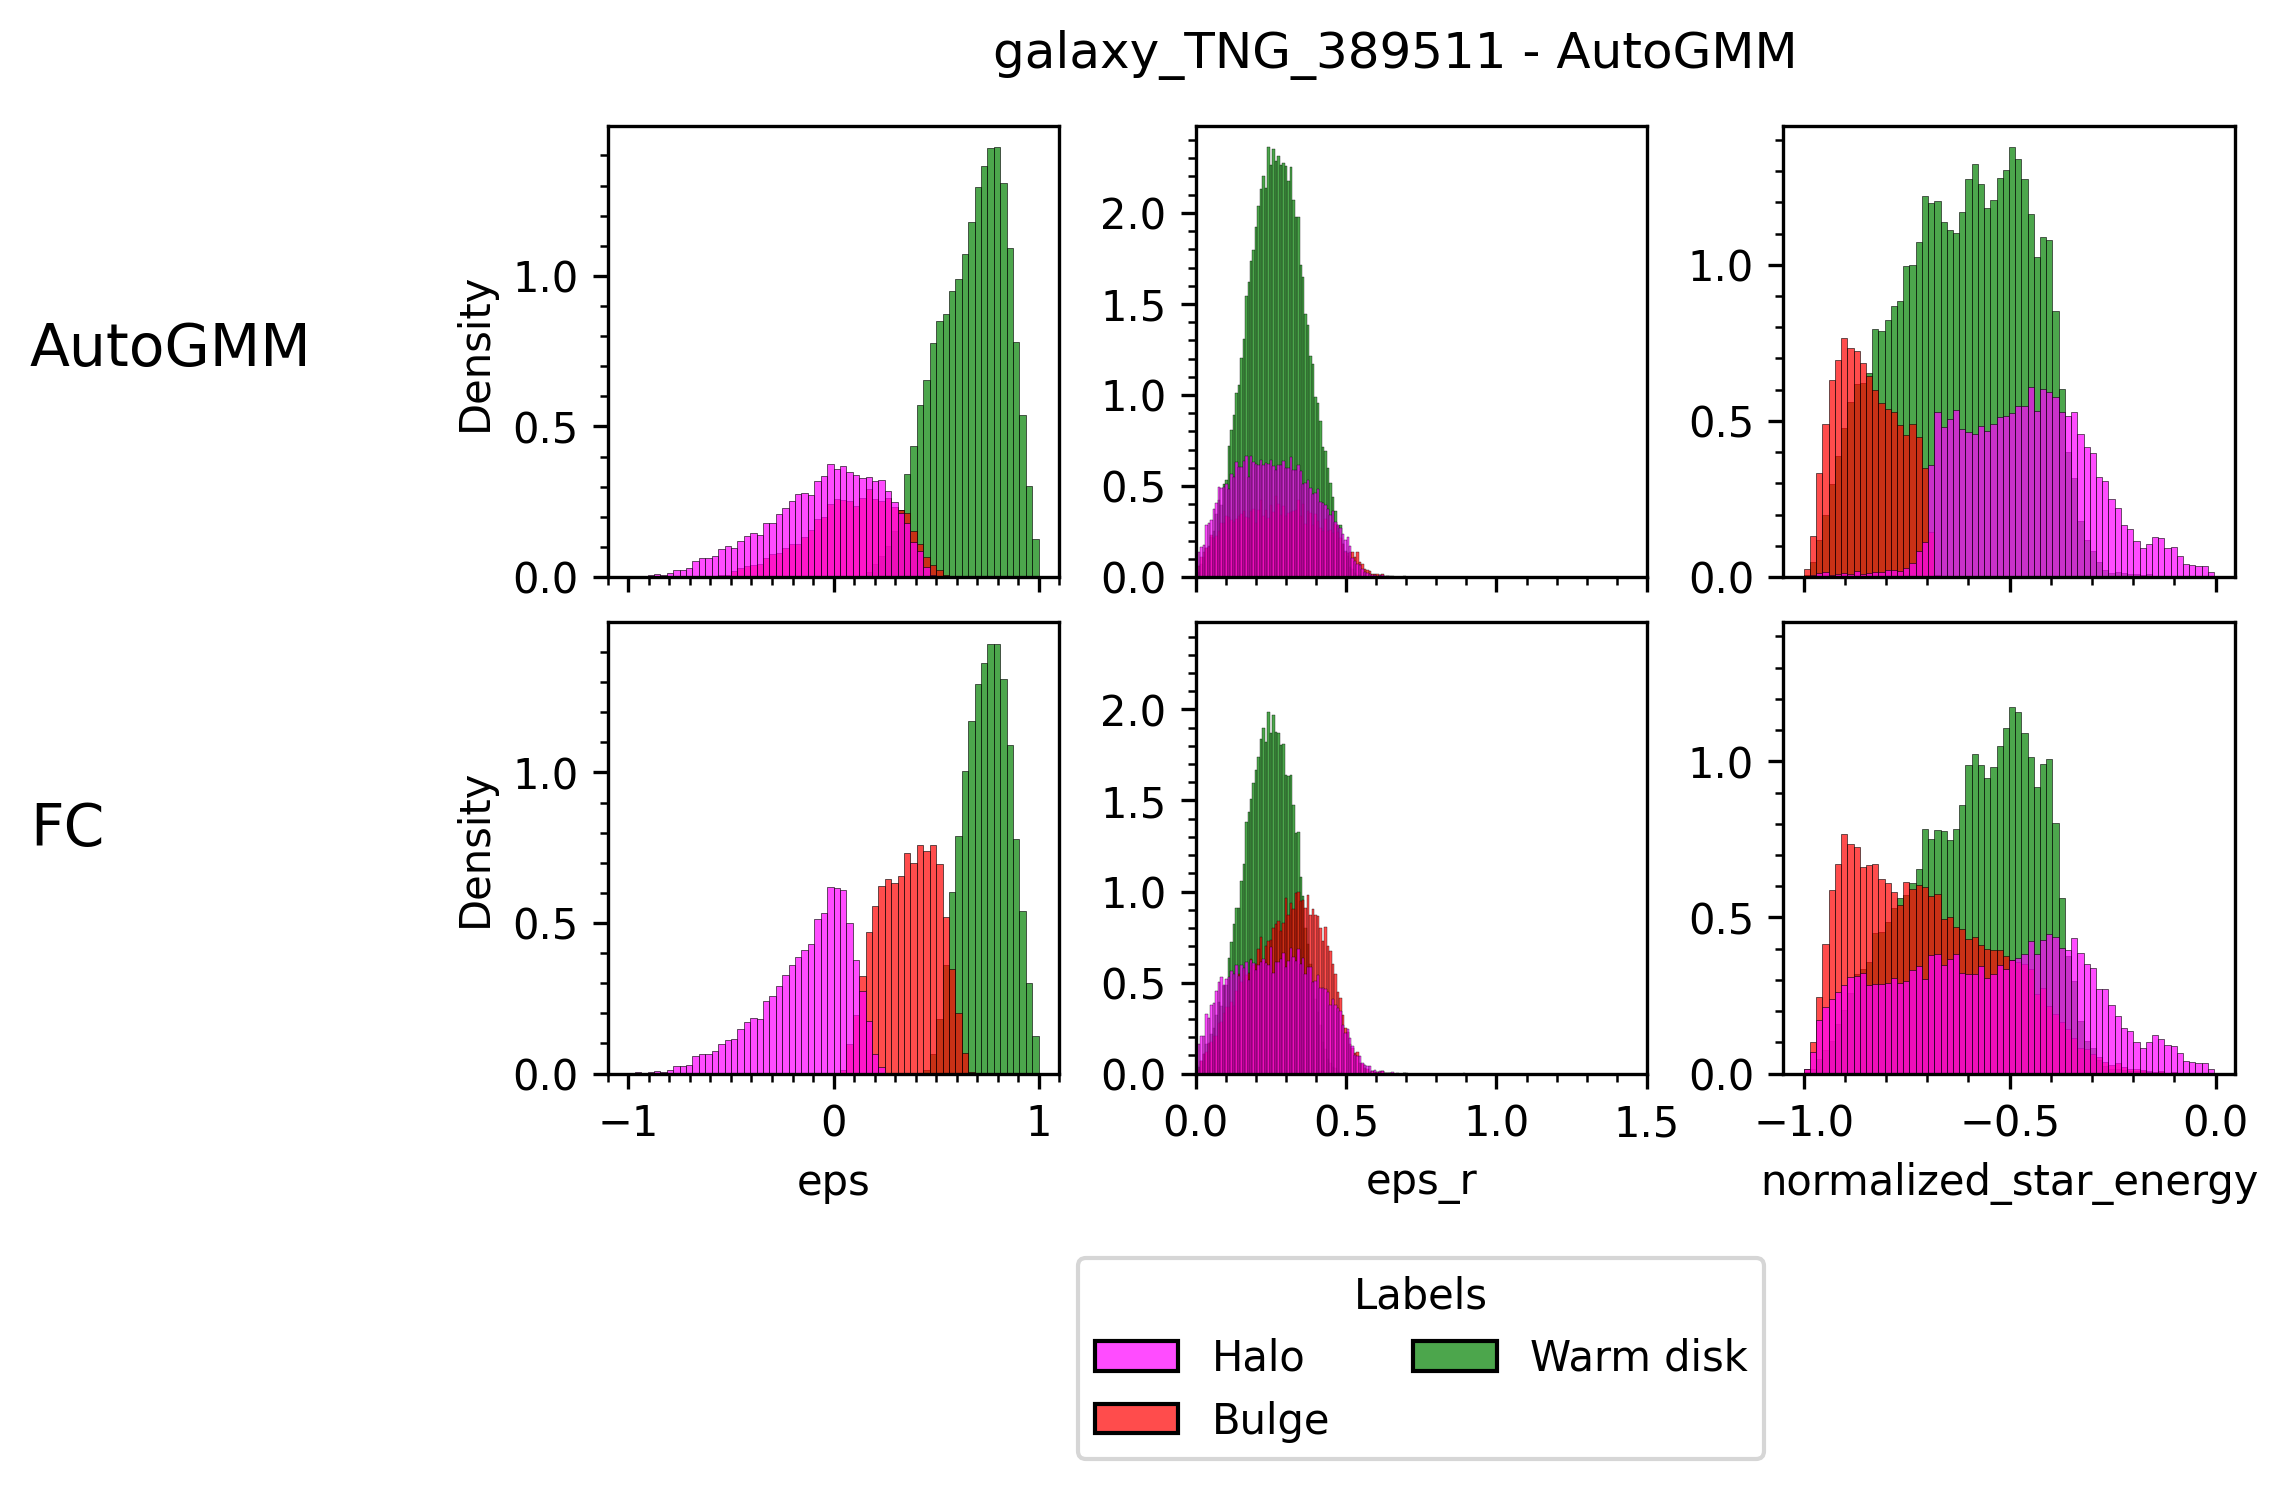
\includegraphics[width=12cm]{fuzzy clustering/figures/galaxy_TNG_389511 - circ histogram.png}
\end{center}

\note{
- Se puede ver de forma aun mas clara el poco impacto que tiene normalized star energy en la clusterizacion realizada por FCM en el histograma, y como esta es mas relevante en agmm \\
}

\end{frame}
\fi


\iflong
\begin{frame}
\frametitle{AGMM: Detección de $>=$2 componentes}

% similar a lo de la seccion anterior
% presente en graficas anteriores, pero se ve mas claro en esta

\begin{center}
    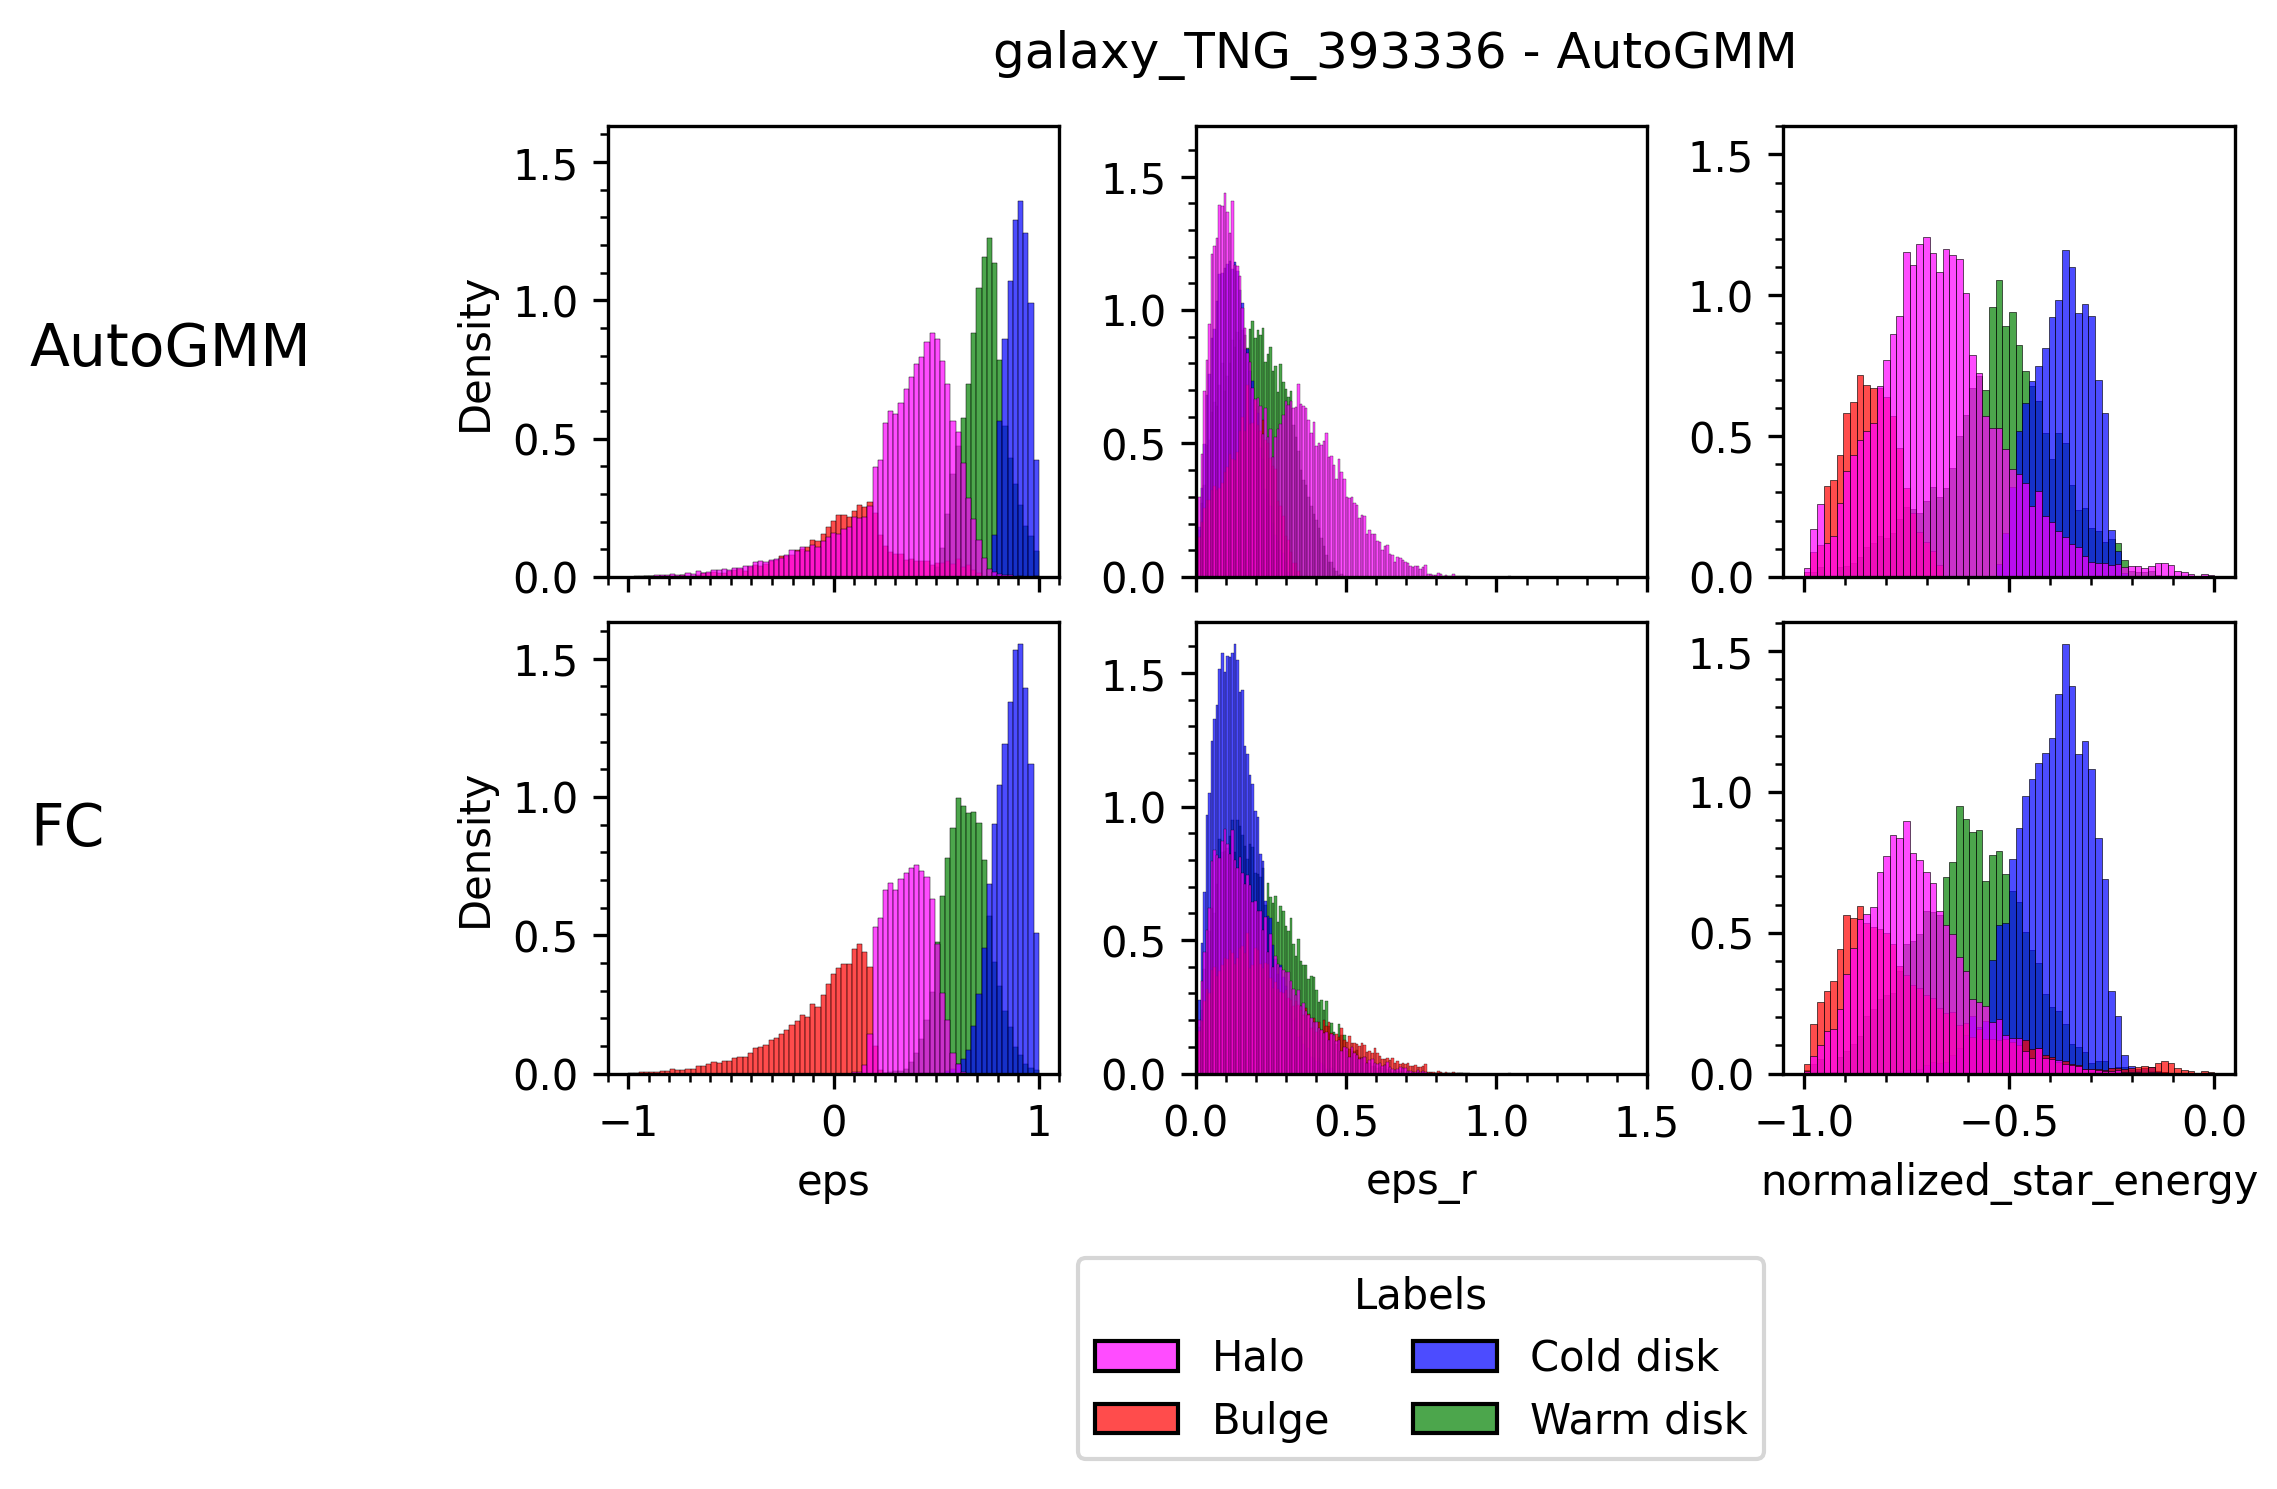
\includegraphics[width=7cm]{fuzzy clustering/figures/galaxy_TNG_393336 - circ histogram.png}
\end{center}

\vspace{-1cm}


\begin{table}
\centering
\begin{tabular}{l|c|c|c|c|}
\cline{3-5}
\multicolumn{2}{c|}{}&center.eps&center.eps\_r&center.normalized\_star\_energy\\
\cline{2-5}
& Bulge & $0.005$ & $0.229$ & $-0.764$\\
\cline{2-5}
& Halo & $0.368$ & $0.197$ & $-0.713$\\
\cline{2-5}
& Warm Disk & $0.632$ & $0.206$ & $-0.586$\\
\cline{2-5}
& Cold Disk & $0.857$ & $0.145$ & $-0.399$\\
\cline{2-5}
\end{tabular}
\end{table}

\note{
- FCM rapida transicion entre Bulge y Halo, por la poca distancia de los centros de cada cluster en normalized\_star\_energy en FCM. Entonces el peso que tendrán las distancias sobre esta feature a cada centro para calcular el valor de pertenencia de la partícula a cada cluster será similar entre ellas \\
- Si miramos la grafica tambien hay una tendencia sobreestimar el Cold Disk por sobre el Warm Disk\\
- Como sus centros en normalized star energy estan un tanto separados va a haber solapamiento entre ambos en eps.\\
- dos zonas de solapamiento, la que warm disk es mayor y la que cold disk es mayor. En la primera, el corte en AGMM es mas recto, por lo cual al tener mas fuzzines con FCM implica que varias particulas estelares van a estar en el Disco fino en lugar del grueso. Y en la segunda zona AGMM se solapa mas que FCM, por lo que sucede lo mismo, y colabora a que tenga mas densidad el Cold Disk. \\
- Este comportamiento se puede ver en la mayoria de las galaxias de nuestro dataset.
}

\end{frame}
\fi



\iflong
\begin{frame}
\frametitle{AGMM: Eliminación de outliers}
% 
% 

\begin{center}
    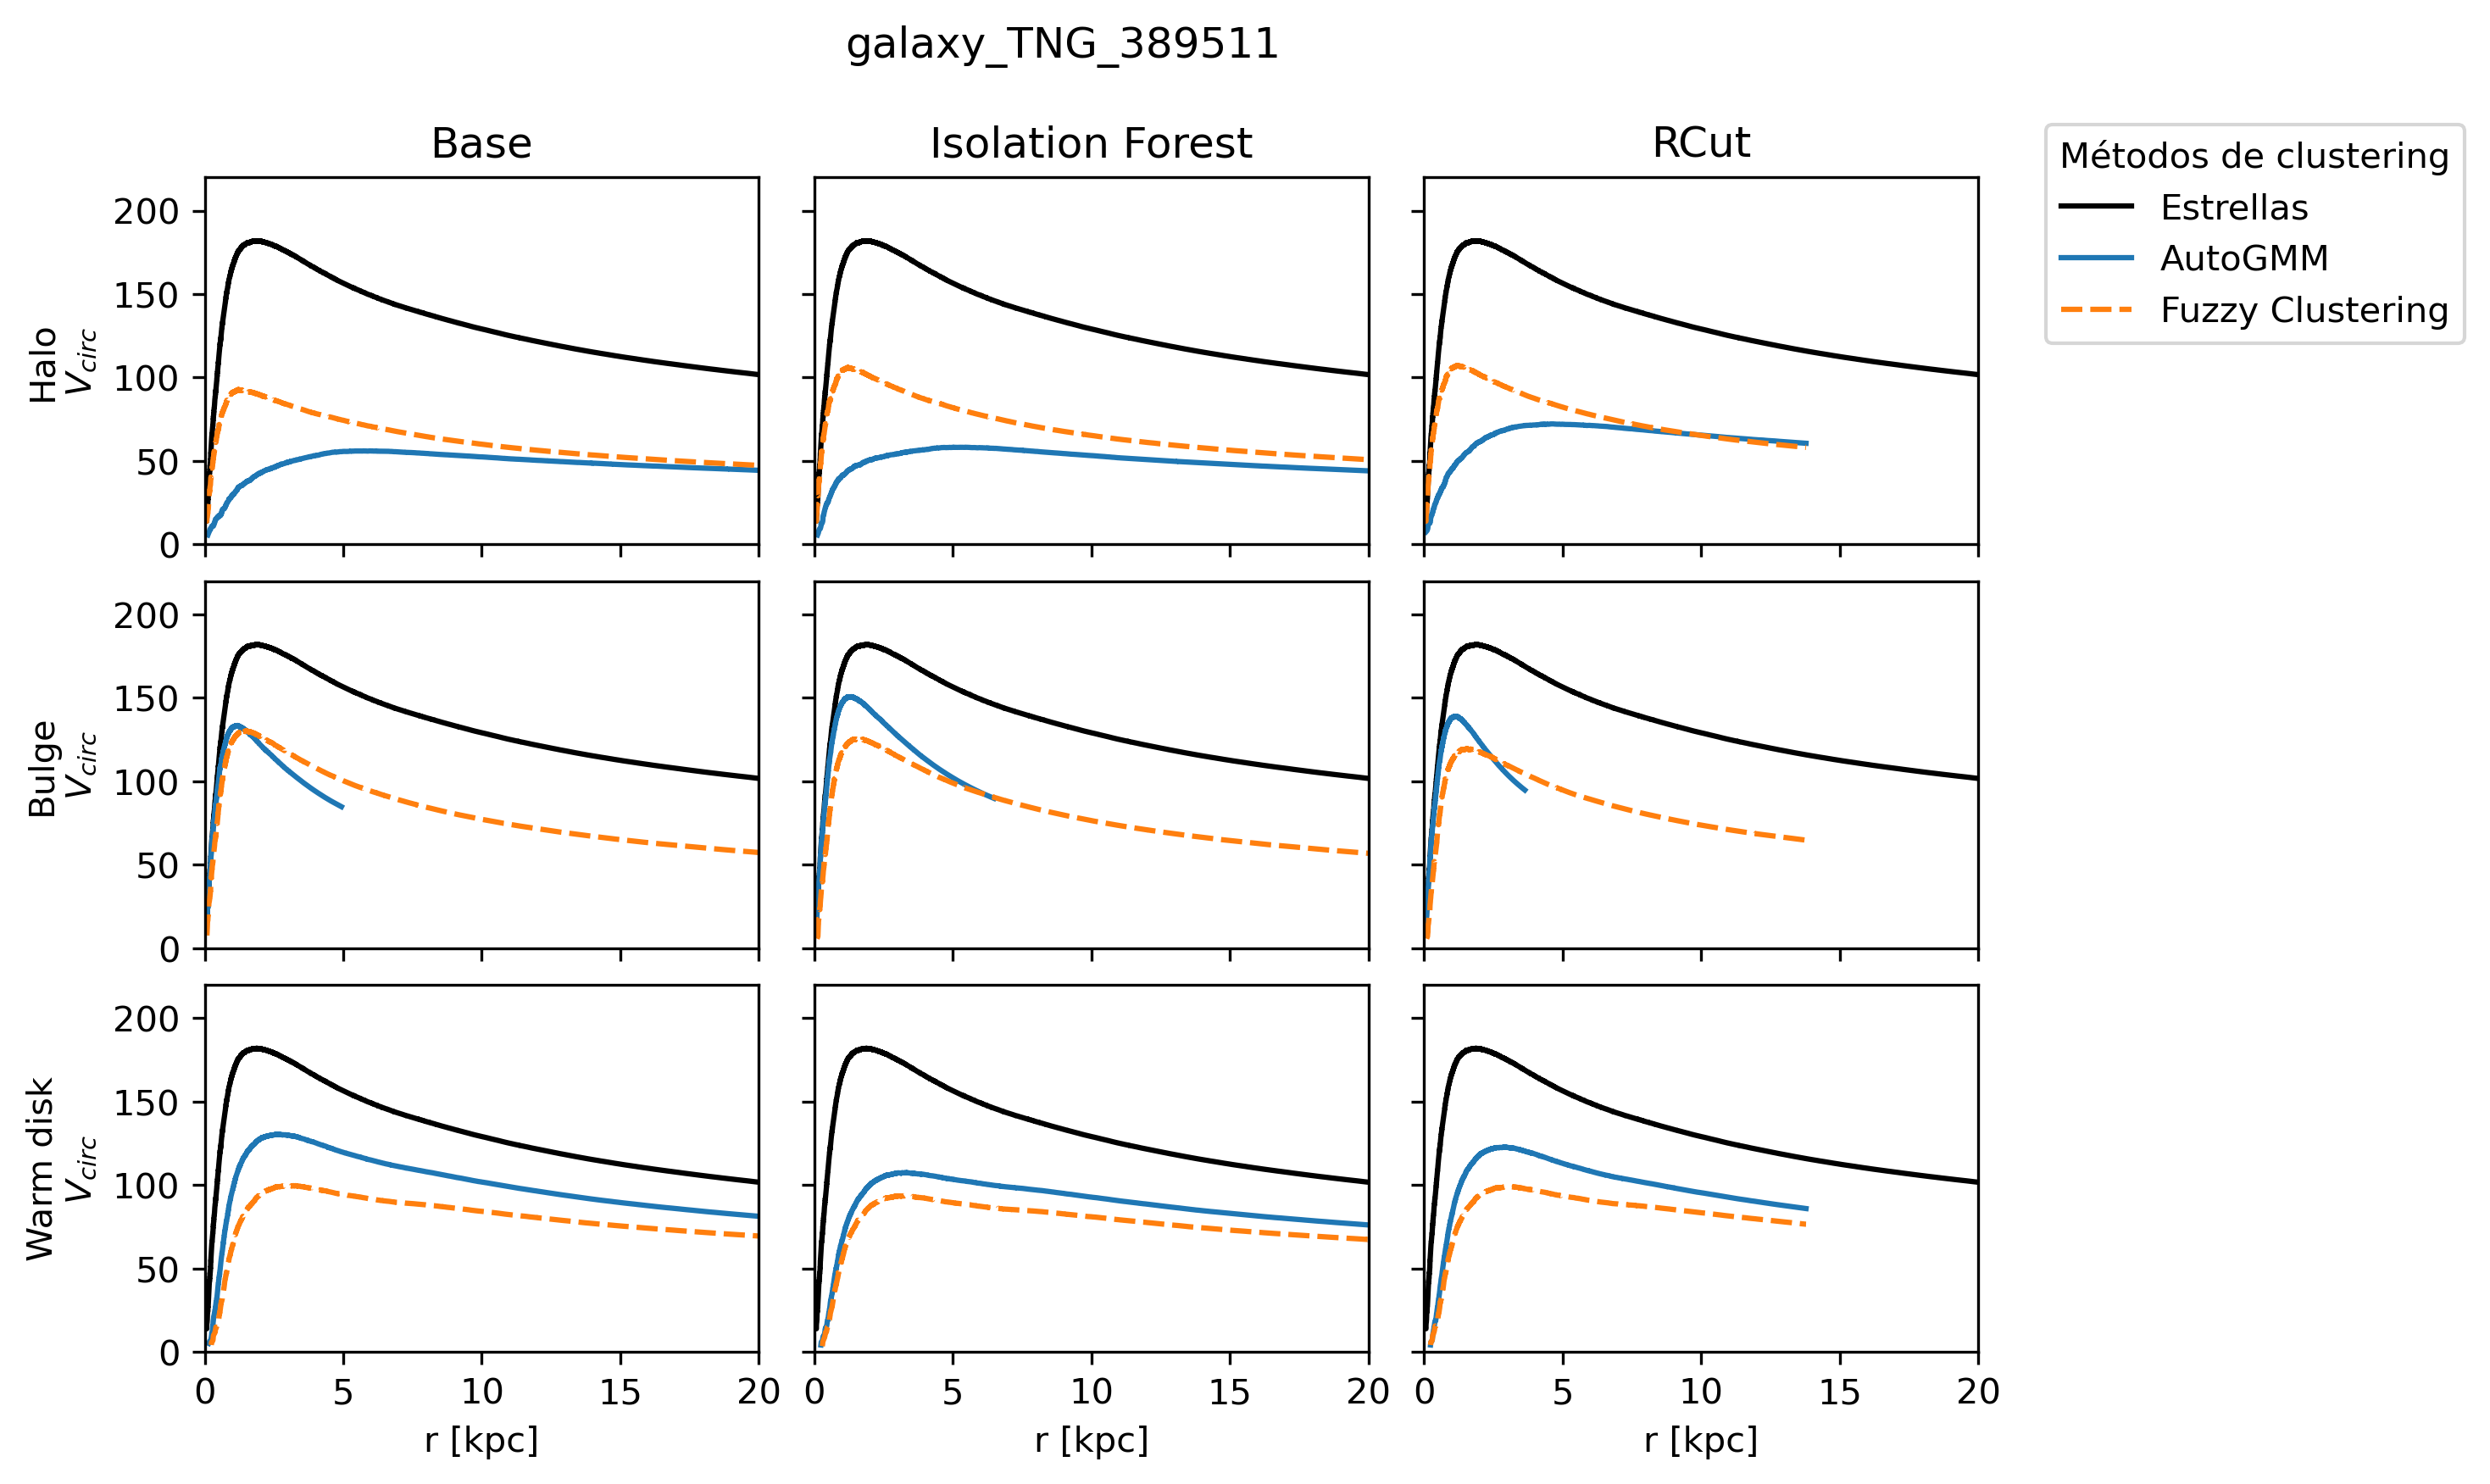
\includegraphics[width=12cm]{fuzzy clustering/figures/galaxy_TNG_389511 - AutoGMM - circ_velocity.png}
\end{center}

\note{
- Eliminar outliers en agmm tiene el mismo problema mencionado en la seccion anterior (n componentes) \\
- al igual que en la seccion anterior, tampoco obtuvimos diferencias tangibles al remover outliers dada la robustez del metodo
}

\end{frame}
\fi



\begin{frame}
\frametitle{AGMM: Eliminación de outliers}


\begin{columns}
\column{0.5\textwidth}

\begin{center}
    Promedio: 0.698
    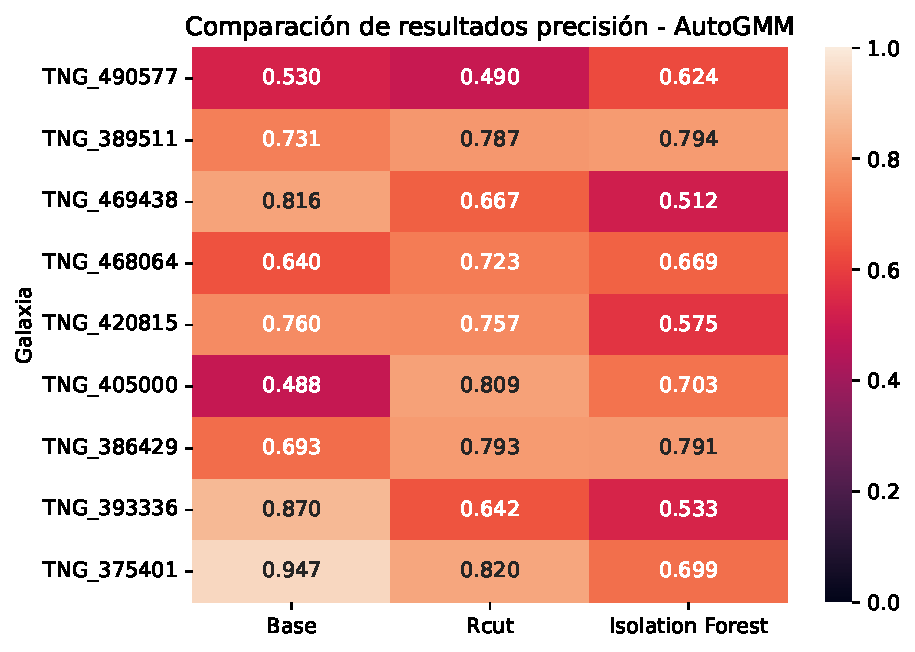
\includegraphics[width=6cm]{clustering jerarquico/figures/precision - agmm.pdf}
\end{center}
\column{0.5\textwidth}
\begin{center}
    Promedio: 0.626
    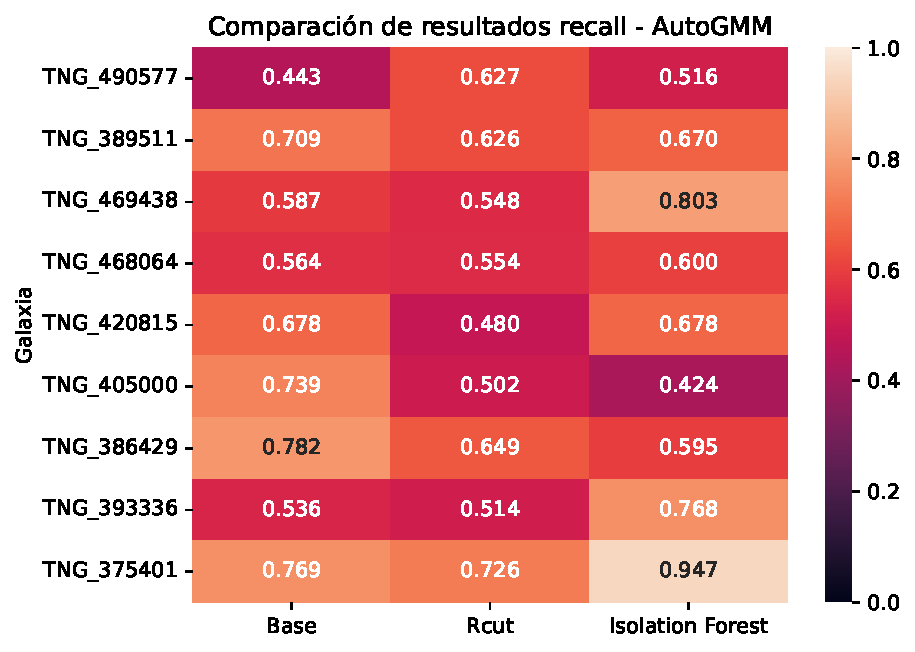
\includegraphics[width=6cm]{clustering jerarquico/figures/recall - agmm.pdf}
\end{center}
\end{columns}

\note{
%- Eliminar outliers en agmm tiene el mismo problema mencionado en la seccion anterior (n componentes) \\
- al igual que en la seccion anterior, tampoco obtuvimos diferencias tangibles al remover outliers dada la \textbf{robustez del metodo} \\
- \textbf{No es una buena alternativa de agmm}
}


\end{frame}



